\chapter{Results}
Using a simulated environment we evaluate how application performance is impacted when using a network of primary memory devices, where latency will inherently increase with each hop. In this chapter we will first measure what latency behaviour looks like when using one single HMC device, with a single link hop. Then we will increase the number of devices and always use the device at the end of the chain, e.g. when having seven devices we will perform all allocations on the seventh device. We will view these results both from a device and an application perspective. Finally, we present a summary of our findings.

%TODO: A more in depth investigation is needed to understand the results, right now they are more experimental?

%\section{Simulations}
%\bigskip

\section{MCF}
The first application to be run is the, arguably, most memory intensive and latency sensitive benchmark in the SPEC2006 suite - 429.mcf. Figure \ref{Memory-access-429-single}, visualising access times when a single HMC device is being used, shows that there is a lot of latency going on during application run time, even though the only contention available is from its own memory requests. Additionally, there are notable peaks present at precisely 93 ns intervals. In-between the aforementioned peaks the pattern looks quite similar with the differences mostly accredited to resolution in terms of occurrences of requests with specific latency.
\bigskip

\begin{figure}[!ht]
    \centering
    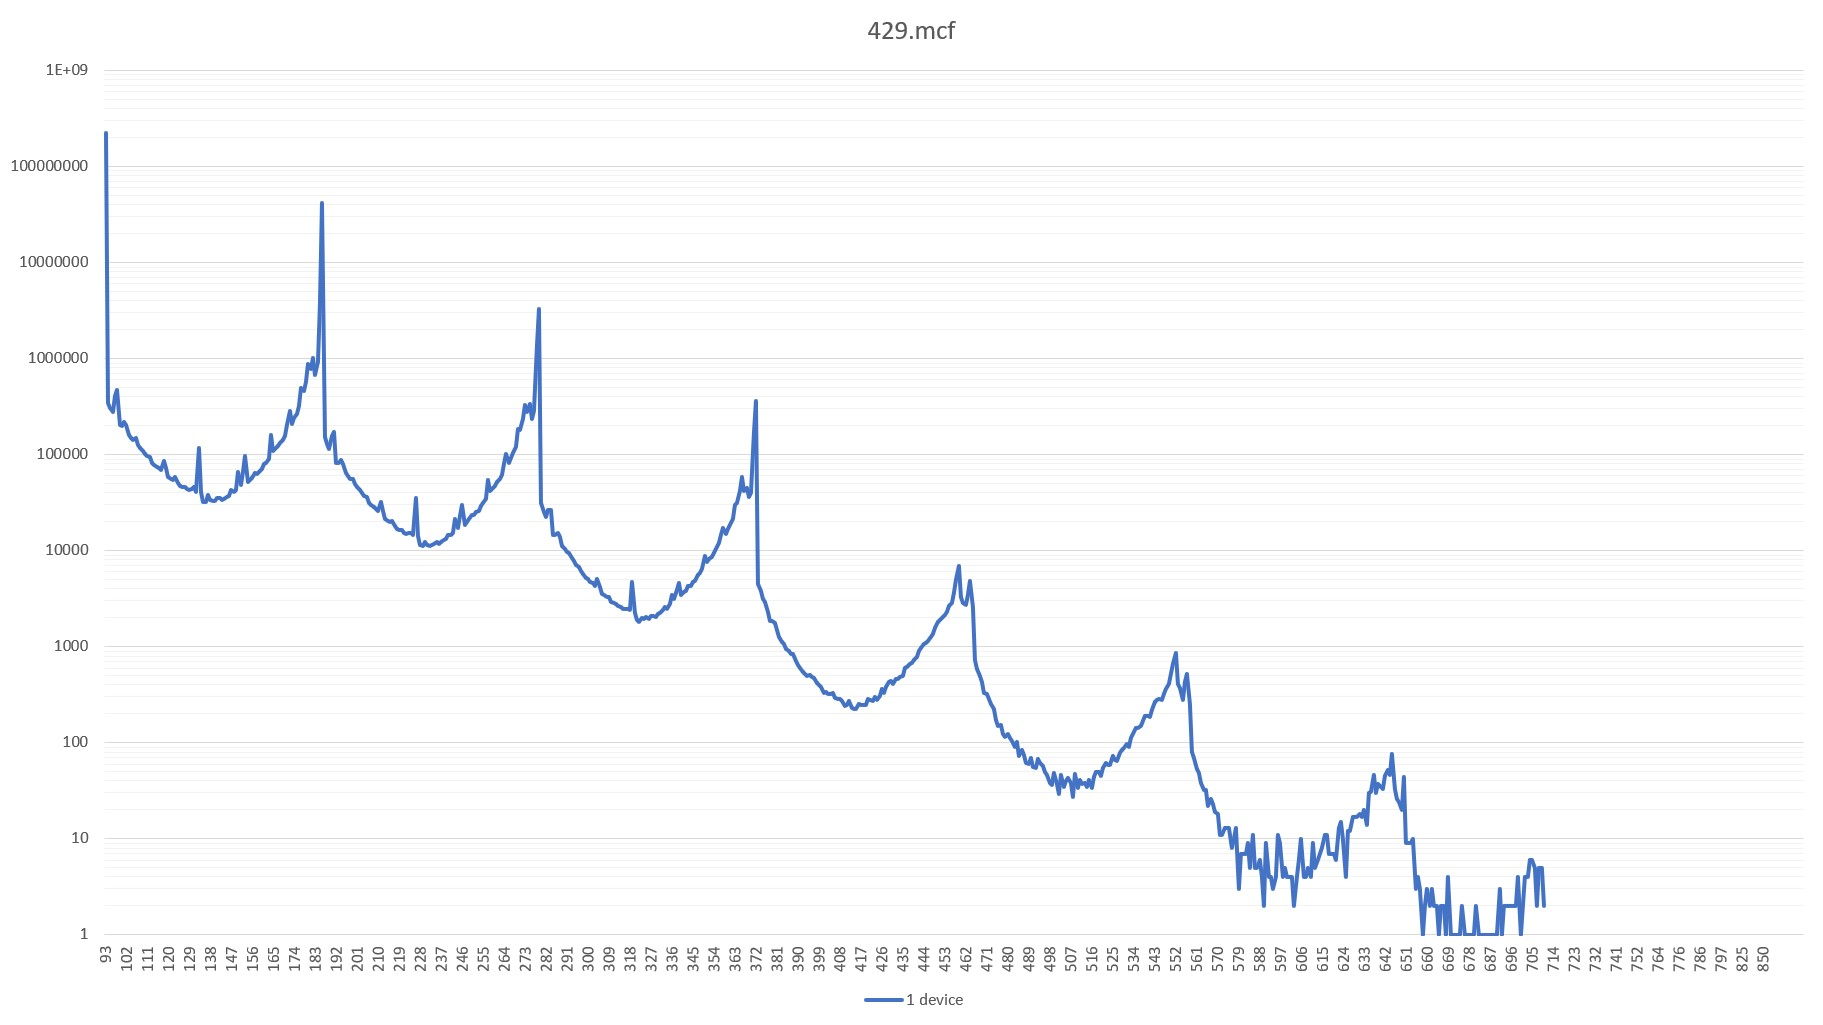
\includegraphics[width=1.0\linewidth]{figure/429-x_4-1.jpg}
    \caption{Access times using one device with two links, running 429.mcf.}
    \label{Memory-access-429-single}
\end{figure}

Adding more devices, and thereby placing data further from the host, will incur greater latencies as seen in figure \ref{Memory-access-429}. However, it can be noted that the peaks all have about the same magnitude and the repeating pattern in between is reminiscent of each other but with a few differences. These variations should be due to contention arising on the links when data to and from far-away devices tries to use the same links. While the links themselves are duplex and allows traffic in both directions simultaneously, the queues can get full if enough data is pushed in a small time frame. This means that contention exists, but should stay virtually unchanged over multiple network hops while running a single application. Comparing the access times of using one device and three, in figure \ref{Memory-access-429-double}, we can see that there are differences in access time distribution, but the main peaks at 93 ns interval remain the same. In addition, ignoring the initial latency we can also calculate that the average latency is the same. 
\bigskip

\begin{figure}[!ht]
    \centering
    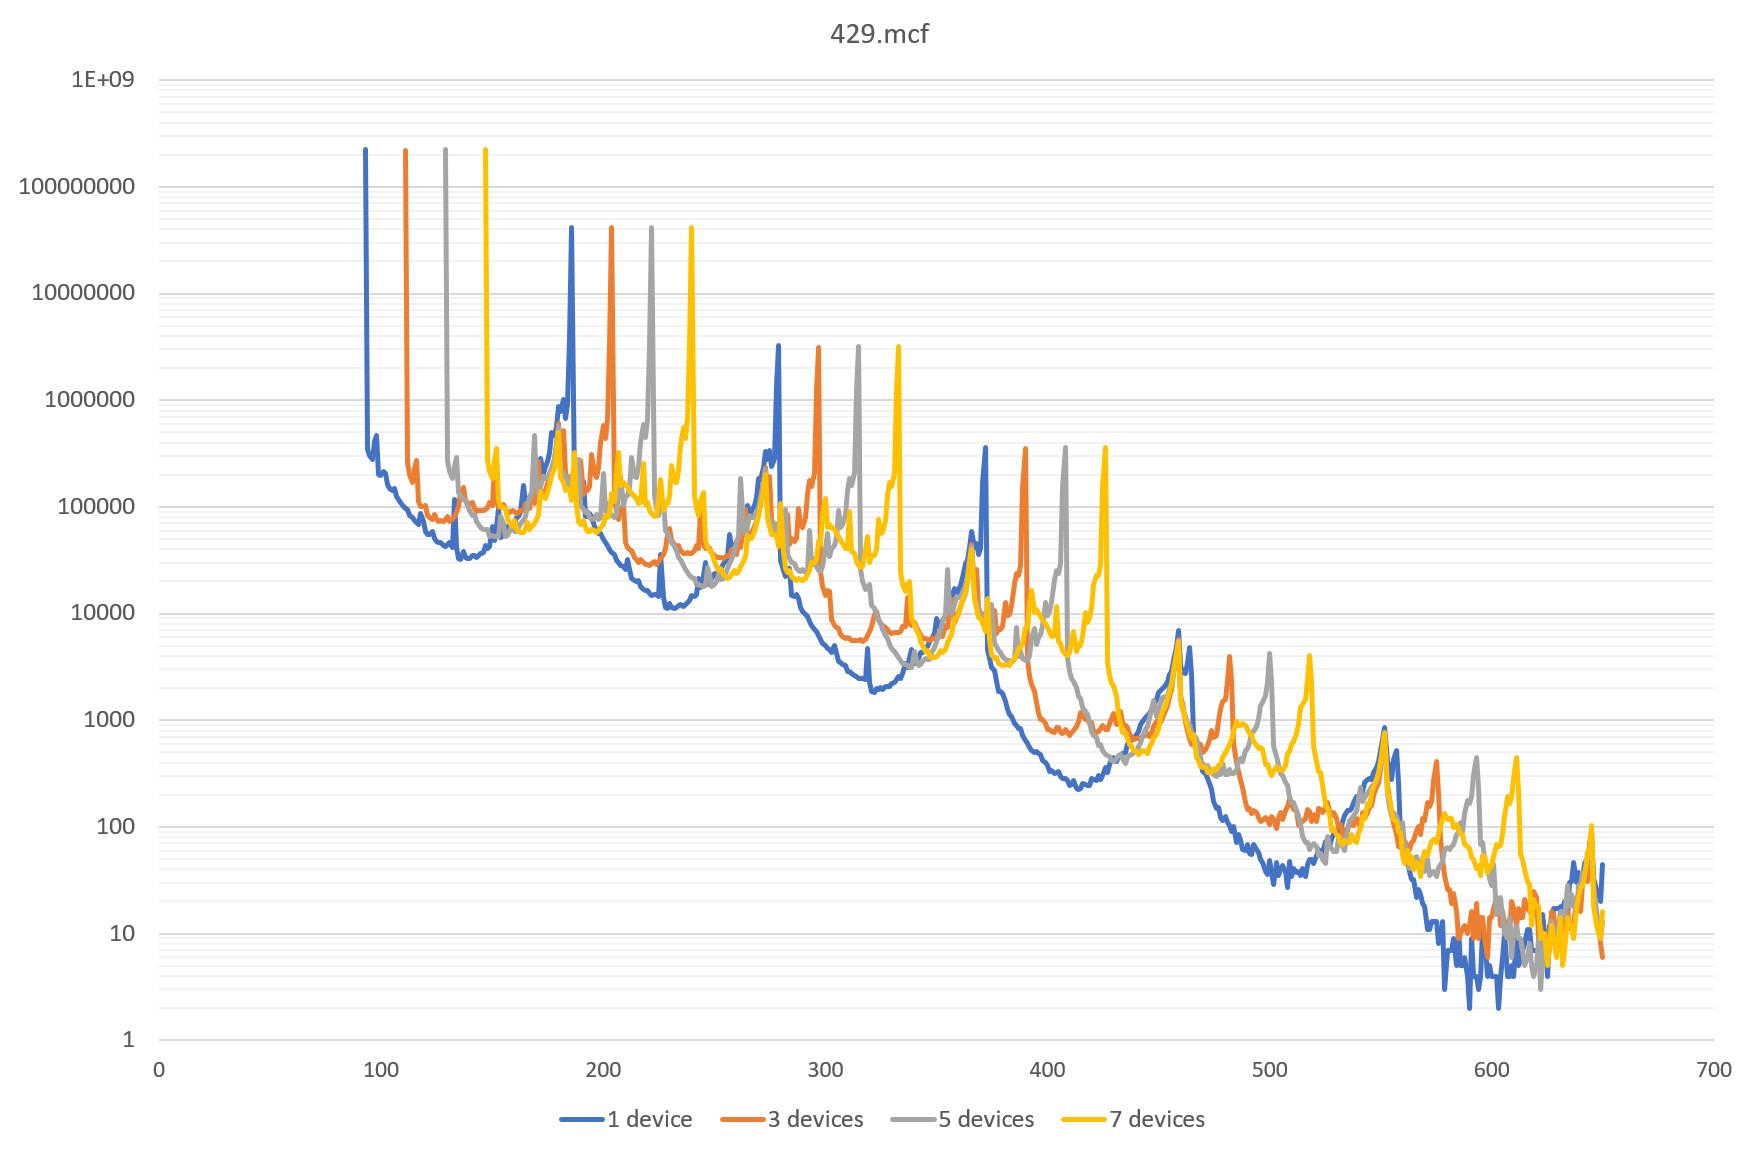
\includegraphics[width=1.0\linewidth]{figure/429-x_4.jpg}
    \caption{Comparing access times when using one, three, five and seven devices.}
    \label{Memory-access-429}
\end{figure}

\begin{figure}[!ht]
    \centering
    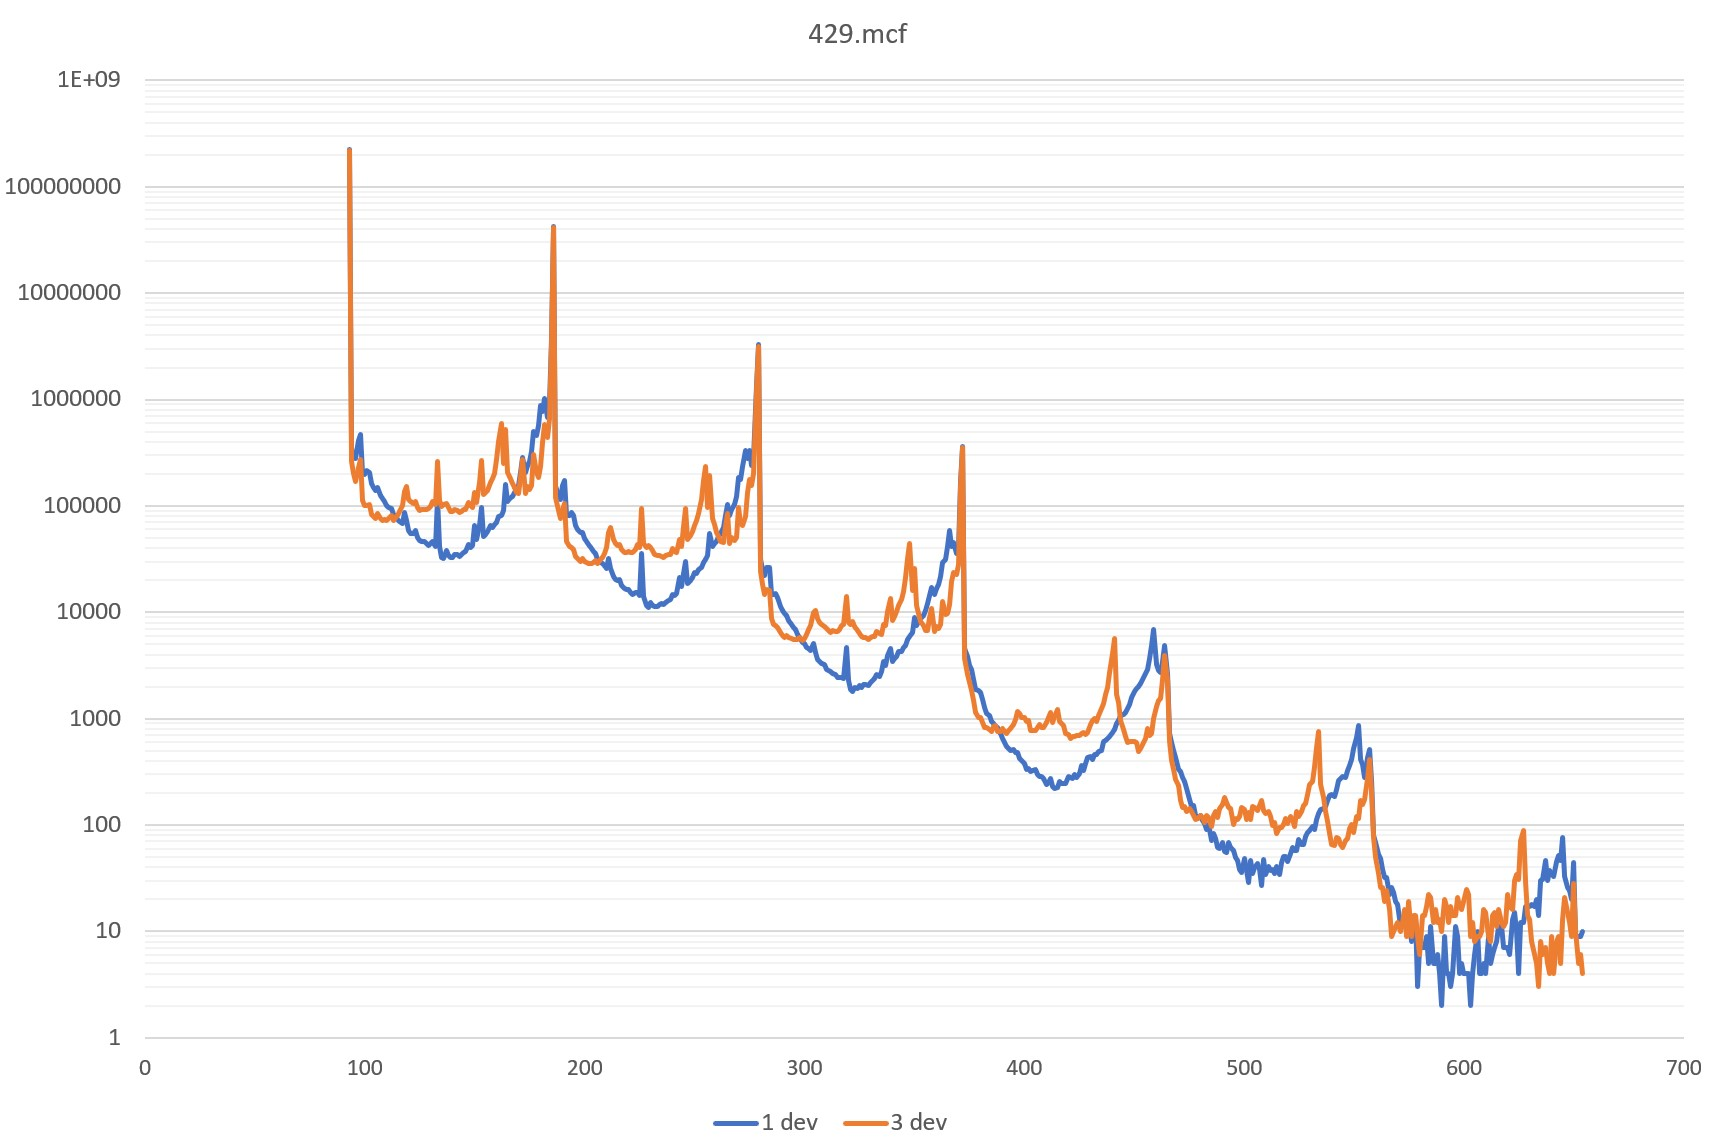
\includegraphics[width=1.0\linewidth]{figure/429-x_4-2.jpg}
    \caption{Access time patterns for one and three devices, where the latter has been adjusted to compensate for initial latency.}
    \label{Memory-access-429-double}
\end{figure}

Next we run using more links between the host and first device, as well as between individual cubes. Specifically, we now simulate using four links instead of the previous two. This should to some extent alleviate the contention issue, but since the access scheme of the links is a simple round robin there might also be some added waiting time before data gets to the host. Running mcf using four active links and more than four devices turned out to take too long time (excess of two months run time) and those simulations were finally terminated.
\bigskip

\begin{figure}[!ht]
    \centering
    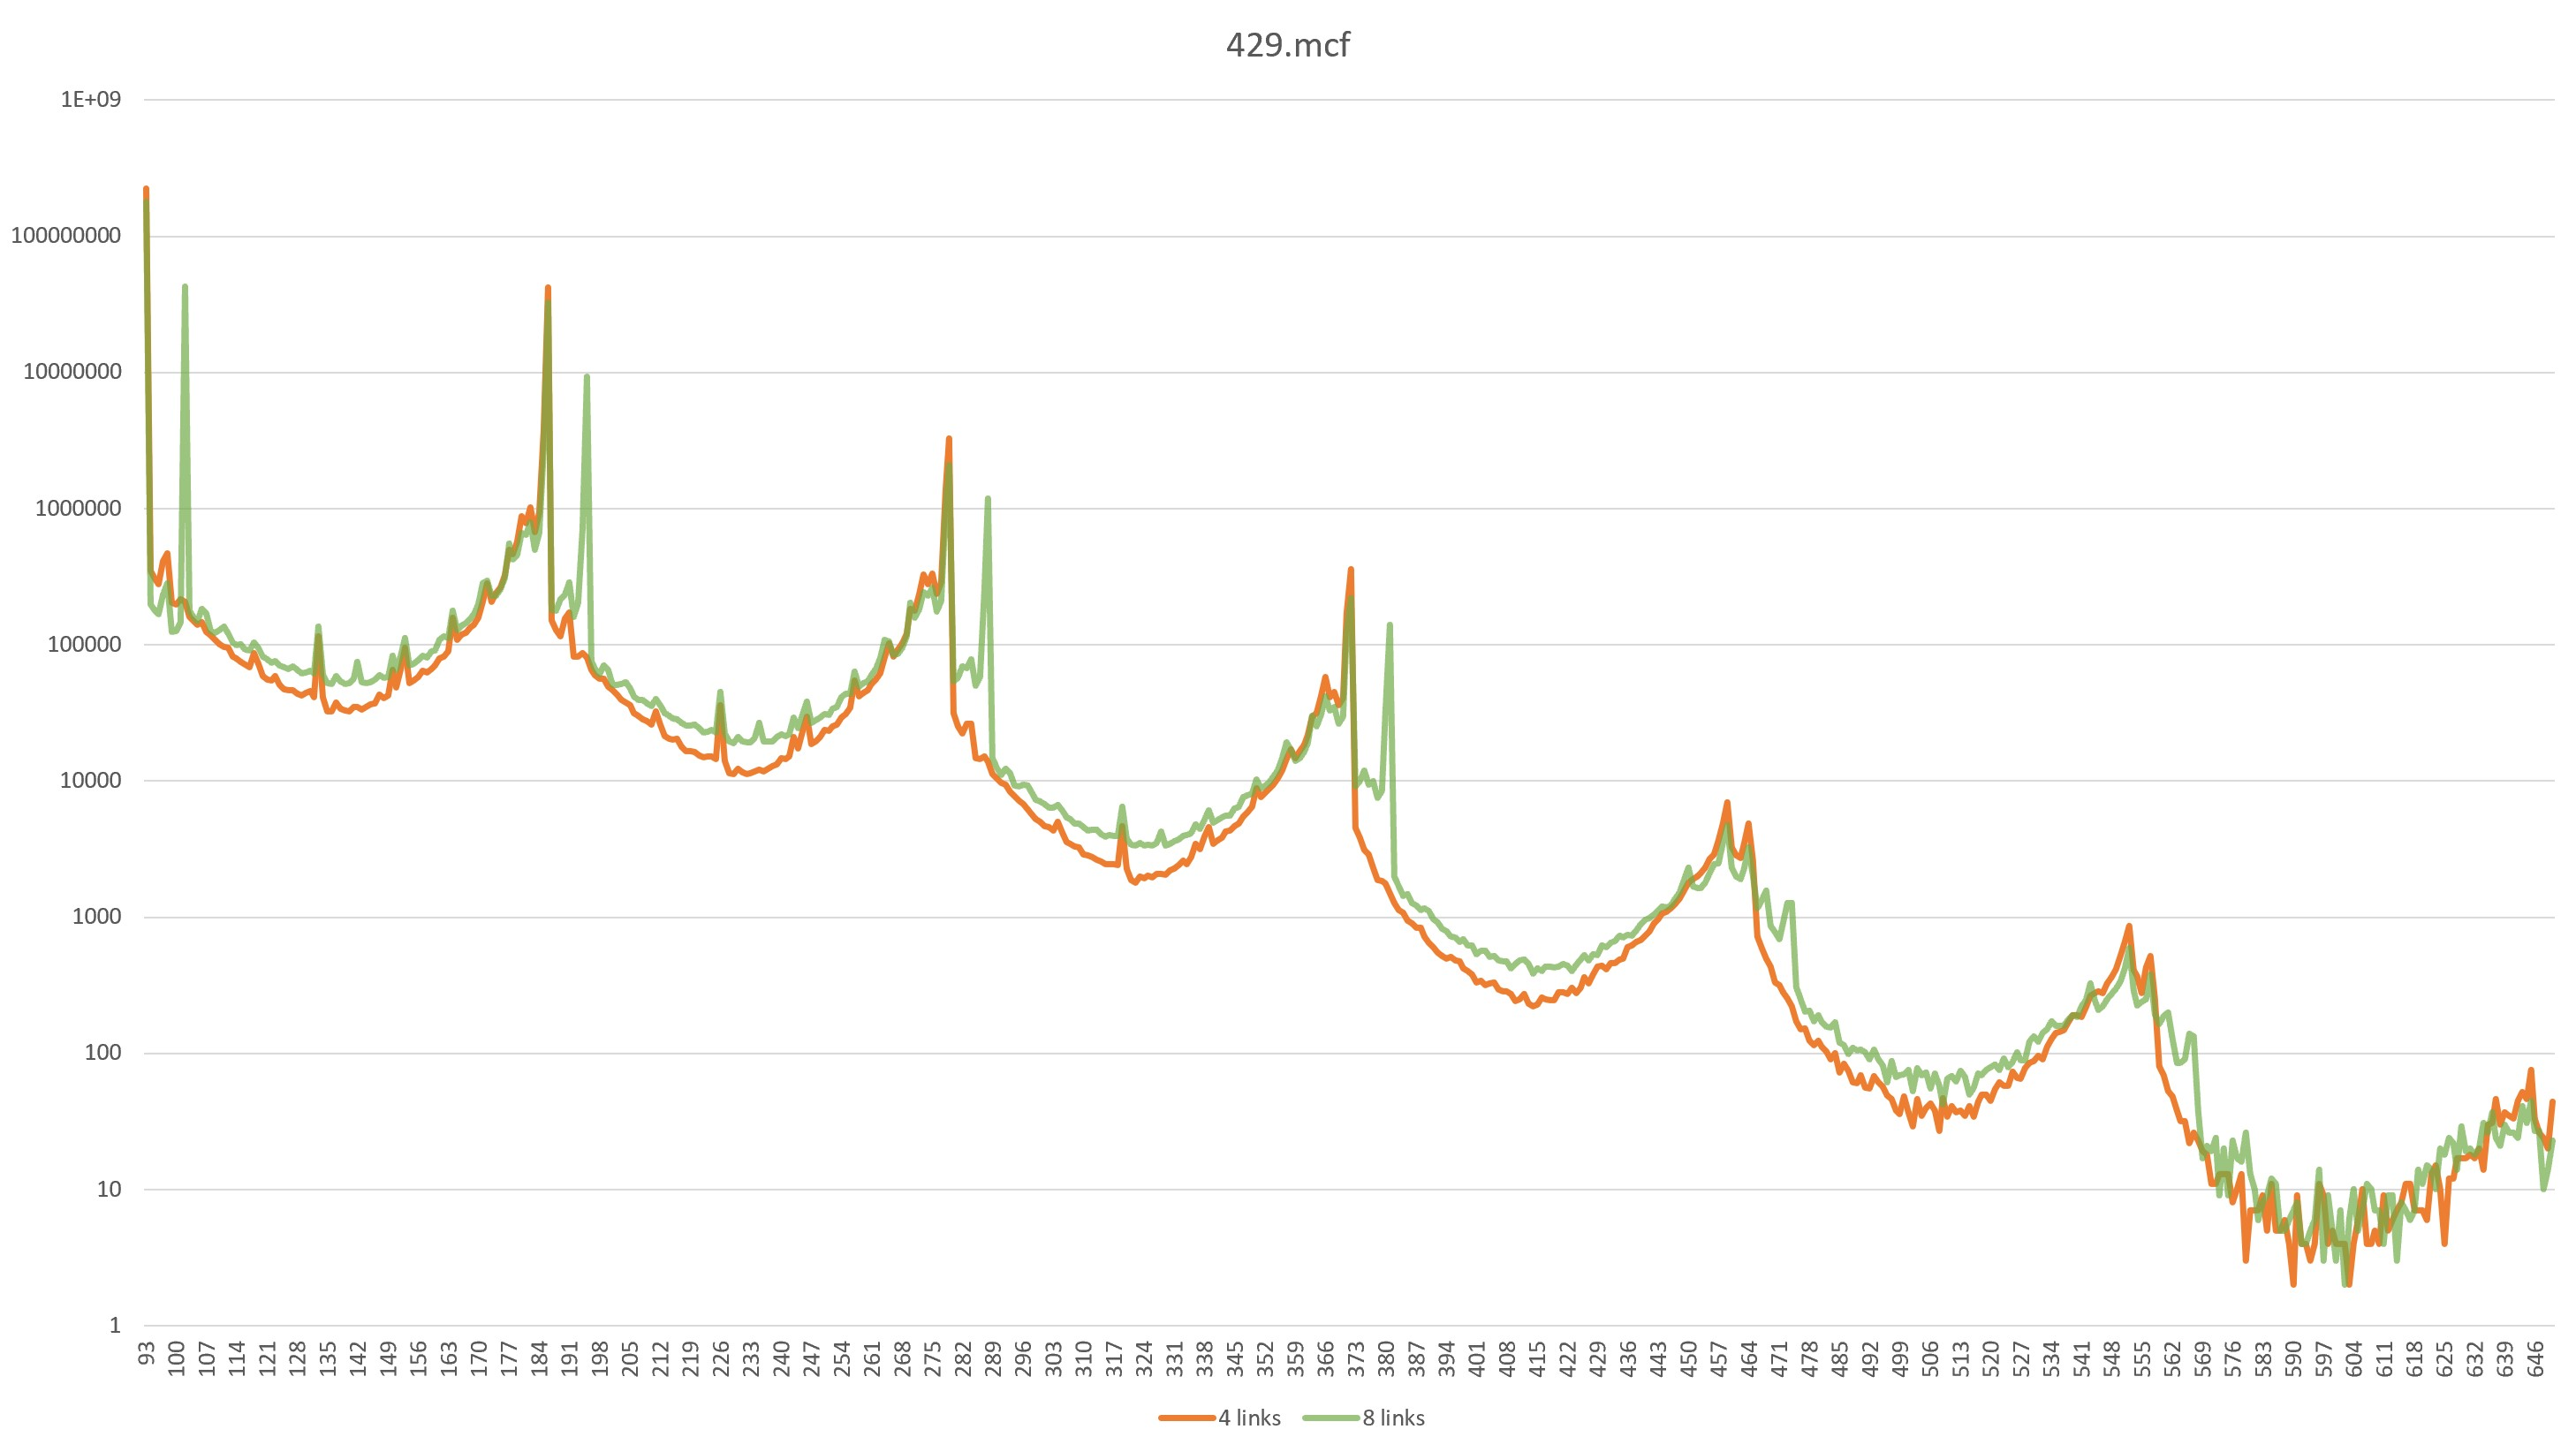
\includegraphics[width=1.0\linewidth]{figure/429-2_4-8.jpg}
    \caption{Part of the access patterns for one and two devices, where the latter has been adjusted to compensate for initial latency.}
    \label{Memory-access-429-link-compare}
\end{figure}

Running mcf using four links produces some odd results. As can be seen in figure \ref{Memory-access-429-link-compare} the access time pattern looks very much like using only two links, but there are new tailing spikes at 9 ns after the bigger peaks. The second spike is a split of the otherwise always present peaks with 93 ns interval, where close to 20\% of those accesses are delayed with 9 ns. If data is sent down a link that is attached to another vault, there will have to be internal routing done by the logic layer which could delay the request. That the delay is 9 ns, which is the latency for an entire transfer over a link, comes down to limitations in the simulators where there are no specific latency set for internal routing. By increasing bandwidth, through increased parallelism, we potentially worsen performance for this single application. However, when using two cubes, i.e. adding a hop, the patterns look almost identical. As such, the added latency of multiple links is cancelled out when having longer network traversal time.
\bigskip

\begin{figure}[!ht]
    \centering
    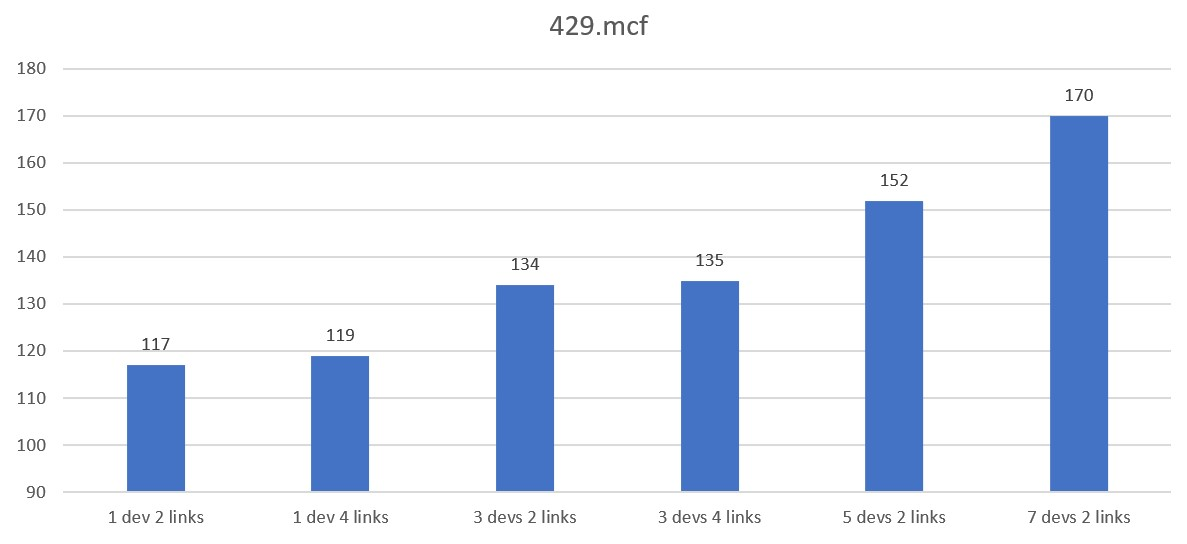
\includegraphics[width=1.0\linewidth]{figure/429-averages.jpg}
    \caption{Comparing access time patterns between configurations.}
    \label{Memory-access-429-average-latency}
\end{figure}

Average latency increases with added network hops, as can be expected, but it also increases somewhat when utilising more parallelism, as seen in figure \ref{Memory-access-429-average-latency}. Although using more than one device masked the specific behaviour from figure \ref{Memory-access-429-link-compare}, the average latency still takes a hit when the application is unable to use the available bandwidth. Comparing average latencies when allocating data on different distances shows that latency increases with 18 ns for every additional hop, which is the round-trip time when each link's latency is 9 ns each way. 

\section{NAMD}
Namd is a mostly compute bound application. This should make access patterns look a little different based on how much data is accessed at a time. In figure \ref{Memory-access-444} we can see what those patterns look like using one, three, five and seven cubes in the network. While there is a pattern between 93 and 186 ns which look quite similar between the configurations, the number of memory requests are too low overall which quickly decreases the resolution and makes patterns almost indiscernible. Many requests do not return immediately, i.e. having a latency of 93 ns, but instead has a higher latency; the most requests are served after 186 ns, which is double that of the minimal possible latency. Namd performs a lot of array lookups and it could be this often-accessed array of subsequent elements we are seeing being used. Additionally, it might be that the introduced MLP hurts performance because the gain of higher bandwidth is outweighed by the overhead of having to wait for internal routing inside the cube. Sadly HMCSim cannot be configured using one single link and thus there is no easy way to verify this claim here.
\bigskip

\begin{figure}[!ht]
    \centering
    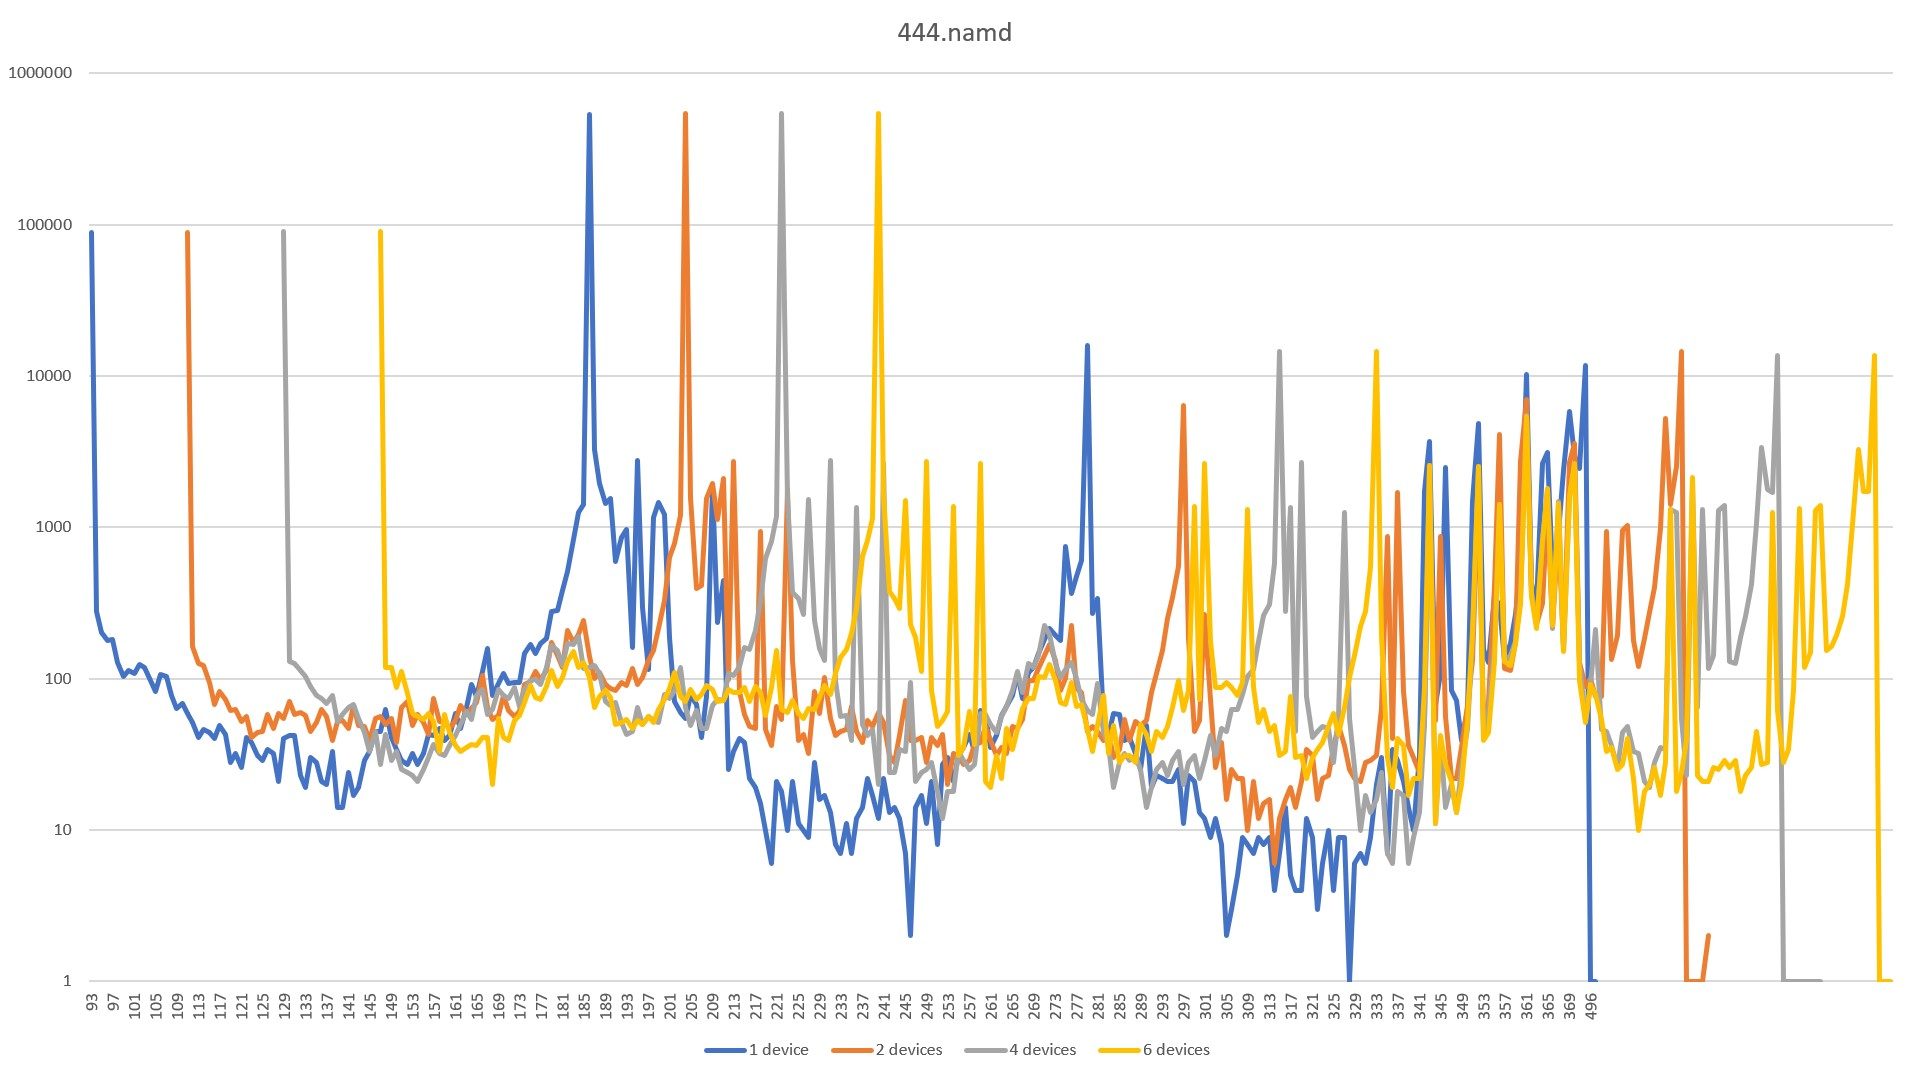
\includegraphics[width=1\linewidth]{figure/444-x_4-1.jpg}
    \caption{Comparing access times when using one, three, five and seven devices.}
    \label{Memory-access-444}
\end{figure}

Adding even more links, using four instead of two, will further hamper the application. Interestingly, the same behaviour as was seen in the mcf results are seen in figure \ref{Memory-access-444-links-compare} as well. There are new peaks added 9 ns after the otherwise normally present peaks. This spike has a much greater impact to this application's average latency compared to mcf, adding five ns as compared to two ns. Because the split spikes represents a larger portion of all memory accesses for namd, it affects the average a lot. In addition, the averages for namd are overall notably higher than those for mcf. However, in the end, as can be seen in figure \ref{Memory-access-444-average-latency}, the biggest hit to performance is taken when introducing new hops.
\bigskip

\begin{figure}[!ht]
    \centering
    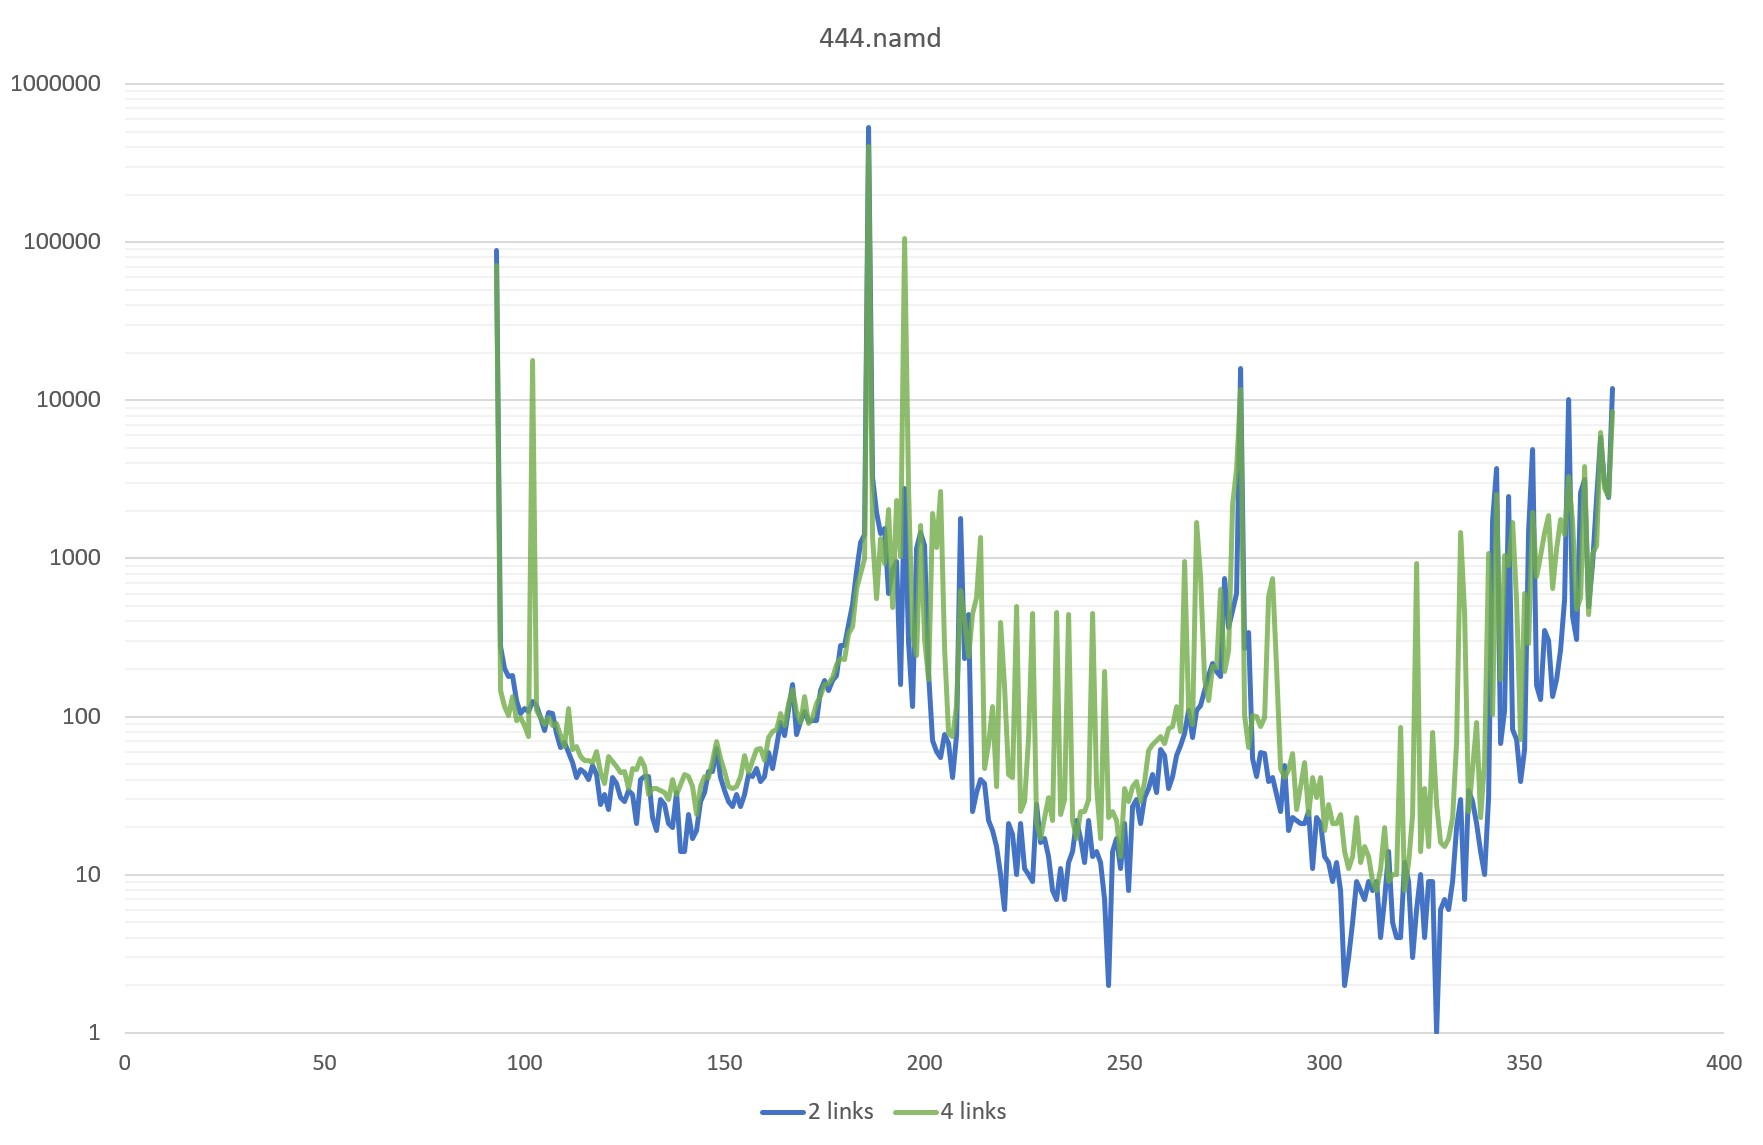
\includegraphics[width=1.0\linewidth]{figure/444-2_4-8.jpg}
    \caption{Comparing latencies when using two and four links using one single device.}
    \label{Memory-access-444-links-compare}
\end{figure}
\begin{figure}[!ht]
    \centering
    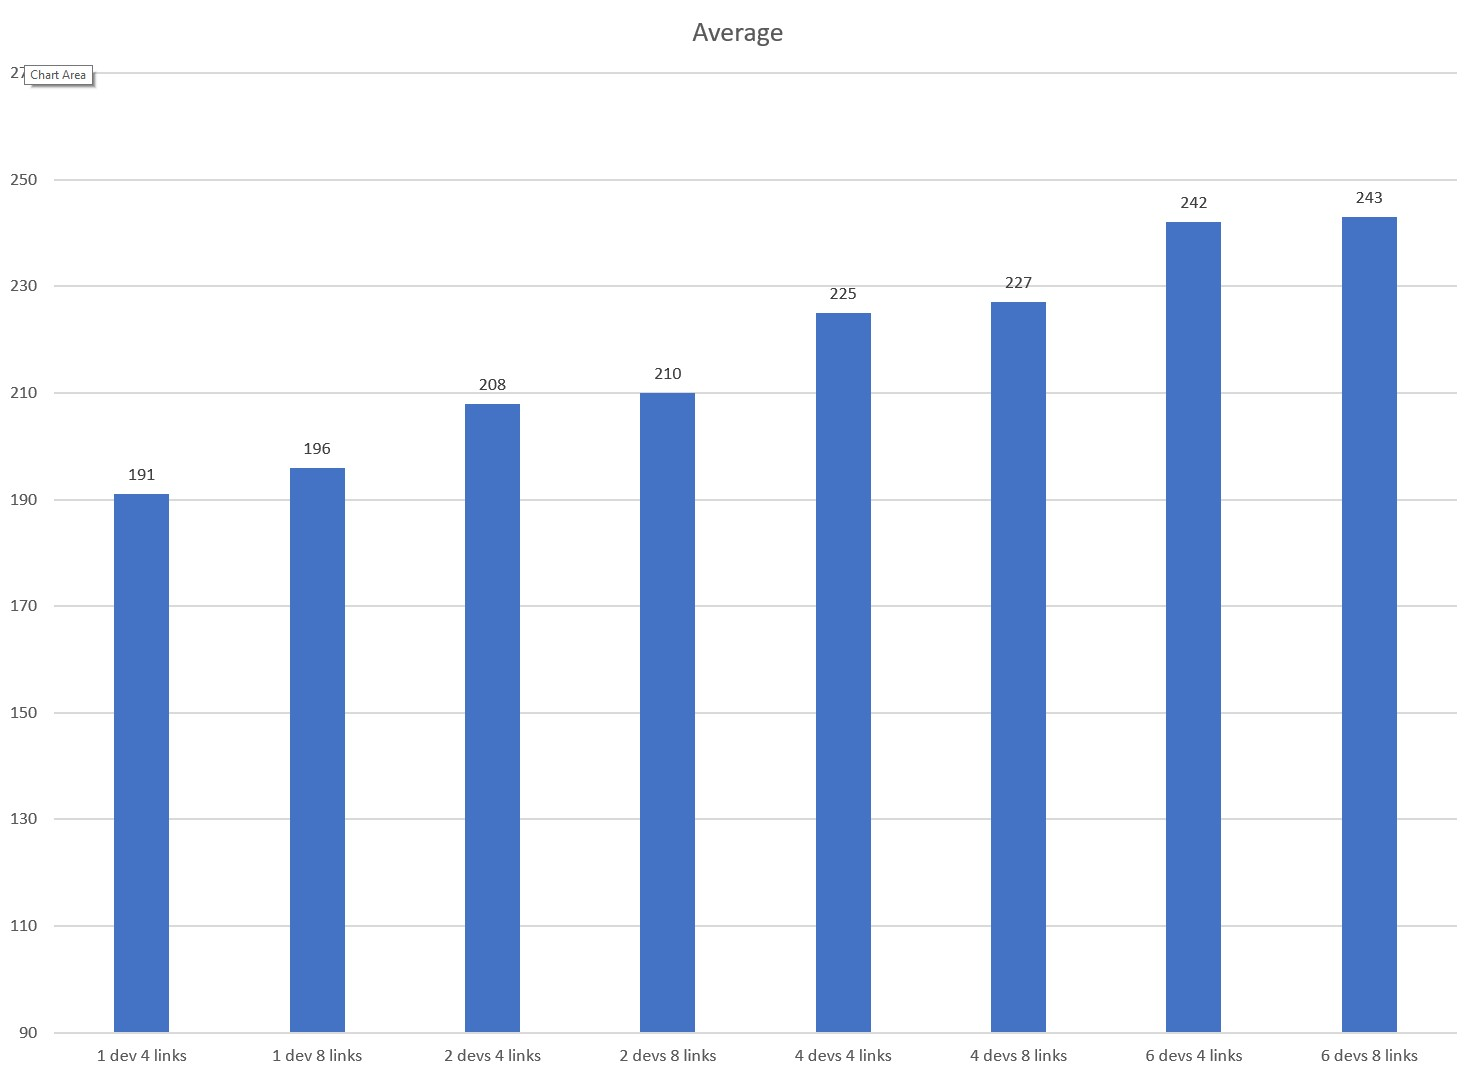
\includegraphics[width=1.0\linewidth]{figure/444_averages.jpg}
    \caption{Comparing average latencies between configurations.}
    \label{Memory-access-444-average-latency}
\end{figure}

\section{SOPLEX}
Soplex is a linear program where every iteration depends on the last. As such, while the application is memory intensive, increased MLP should not yield significant improvements for the general algorithm. However, when starting to look at the average latencies we notice an unexpected result, as seen in figure \ref{Memory-access-450-average-latency}. Having four devices with four links generates, marginally, better results with respect to the average latency. It is hard to determine what exactly made the difference, since, as can be seen in the comparative figure \ref{Memory-access-450-4-dev-4-8-links}, the access patterns between the two look more or less identical. This resembles what other applications have showcased, that increased hop distance does not create the latencies otherwise seen when using just one device. In addition, the averages are rounded down as well and the real difference isn't that big -- the values have been close to 122 but rounded differently. In the end, this result could be interpreted as being within the margin of error and the real results be seen as more or less equal.

\begin{figure}[!ht]
    \centering
    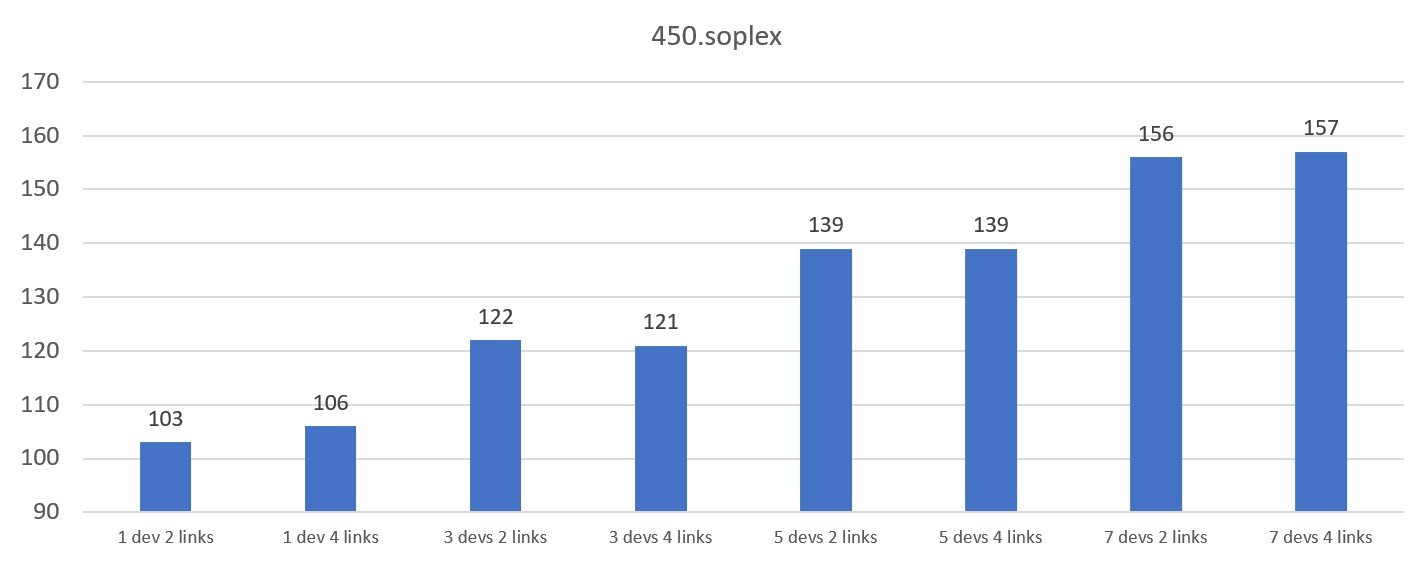
\includegraphics[width=1.0\linewidth]{figure/450-averages.jpg}
    \caption{Comparing average latencies between configurations.}
    \label{Memory-access-450-average-latency}
\end{figure}

\begin{figure}[!ht]
    \centering
    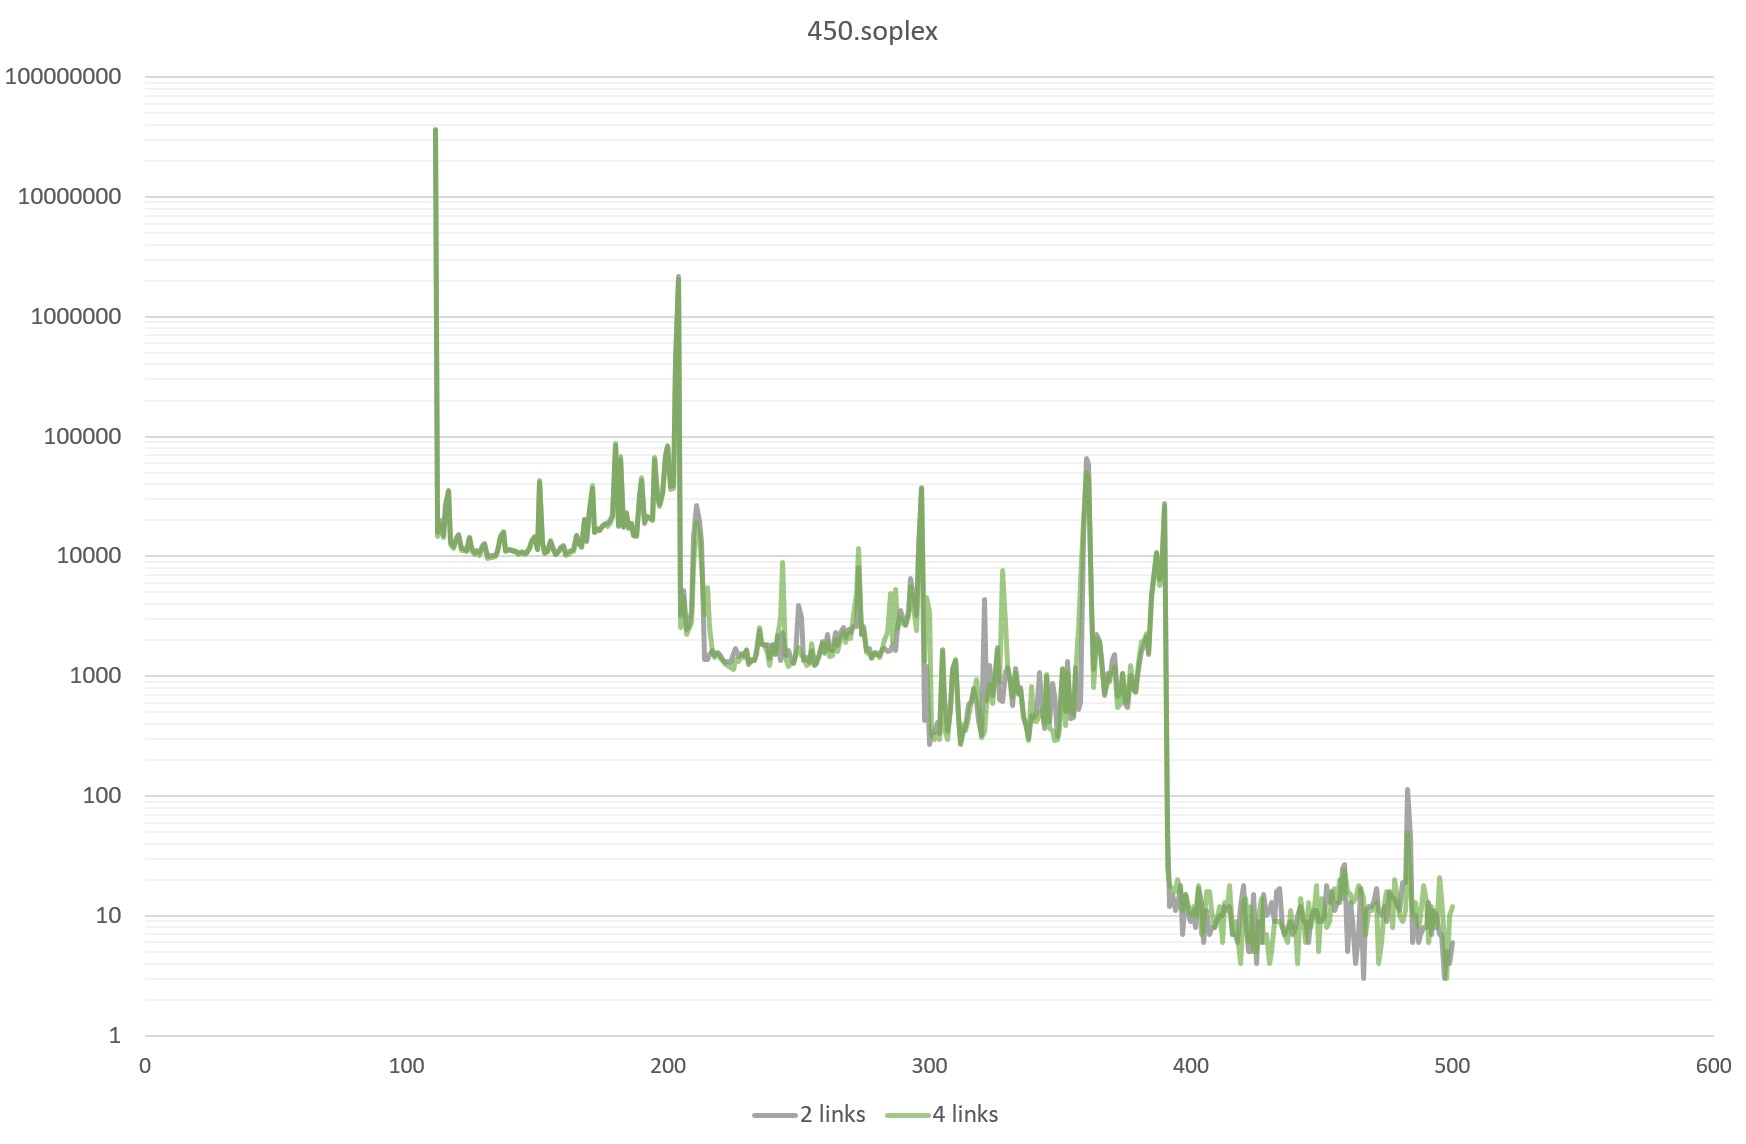
\includegraphics[width=1.0\linewidth]{figure/450-4_4-8.jpg}
    \caption{Nearly identical latencies with two and four links when using three devices.}
    \label{Memory-access-450-4-dev-4-8-links}
\end{figure}

Otherwise we see a familiar pattern in figure \ref{Memory-access-450-2-dev-4-8-links}, where additional spikes arise 9 ns behind the largest peaks when using four links and allocating data close to the processor. This also affects the average latency in this configuration, making it three ns slower compared to using only two links due to this phenomena. As seen before, however, this behaviour seems to be isolated to having more links close to the processor. Apart from this it does not look like soplex neither suffers nor gains from having access to more links. 

\begin{figure}[!ht]
    \centering
    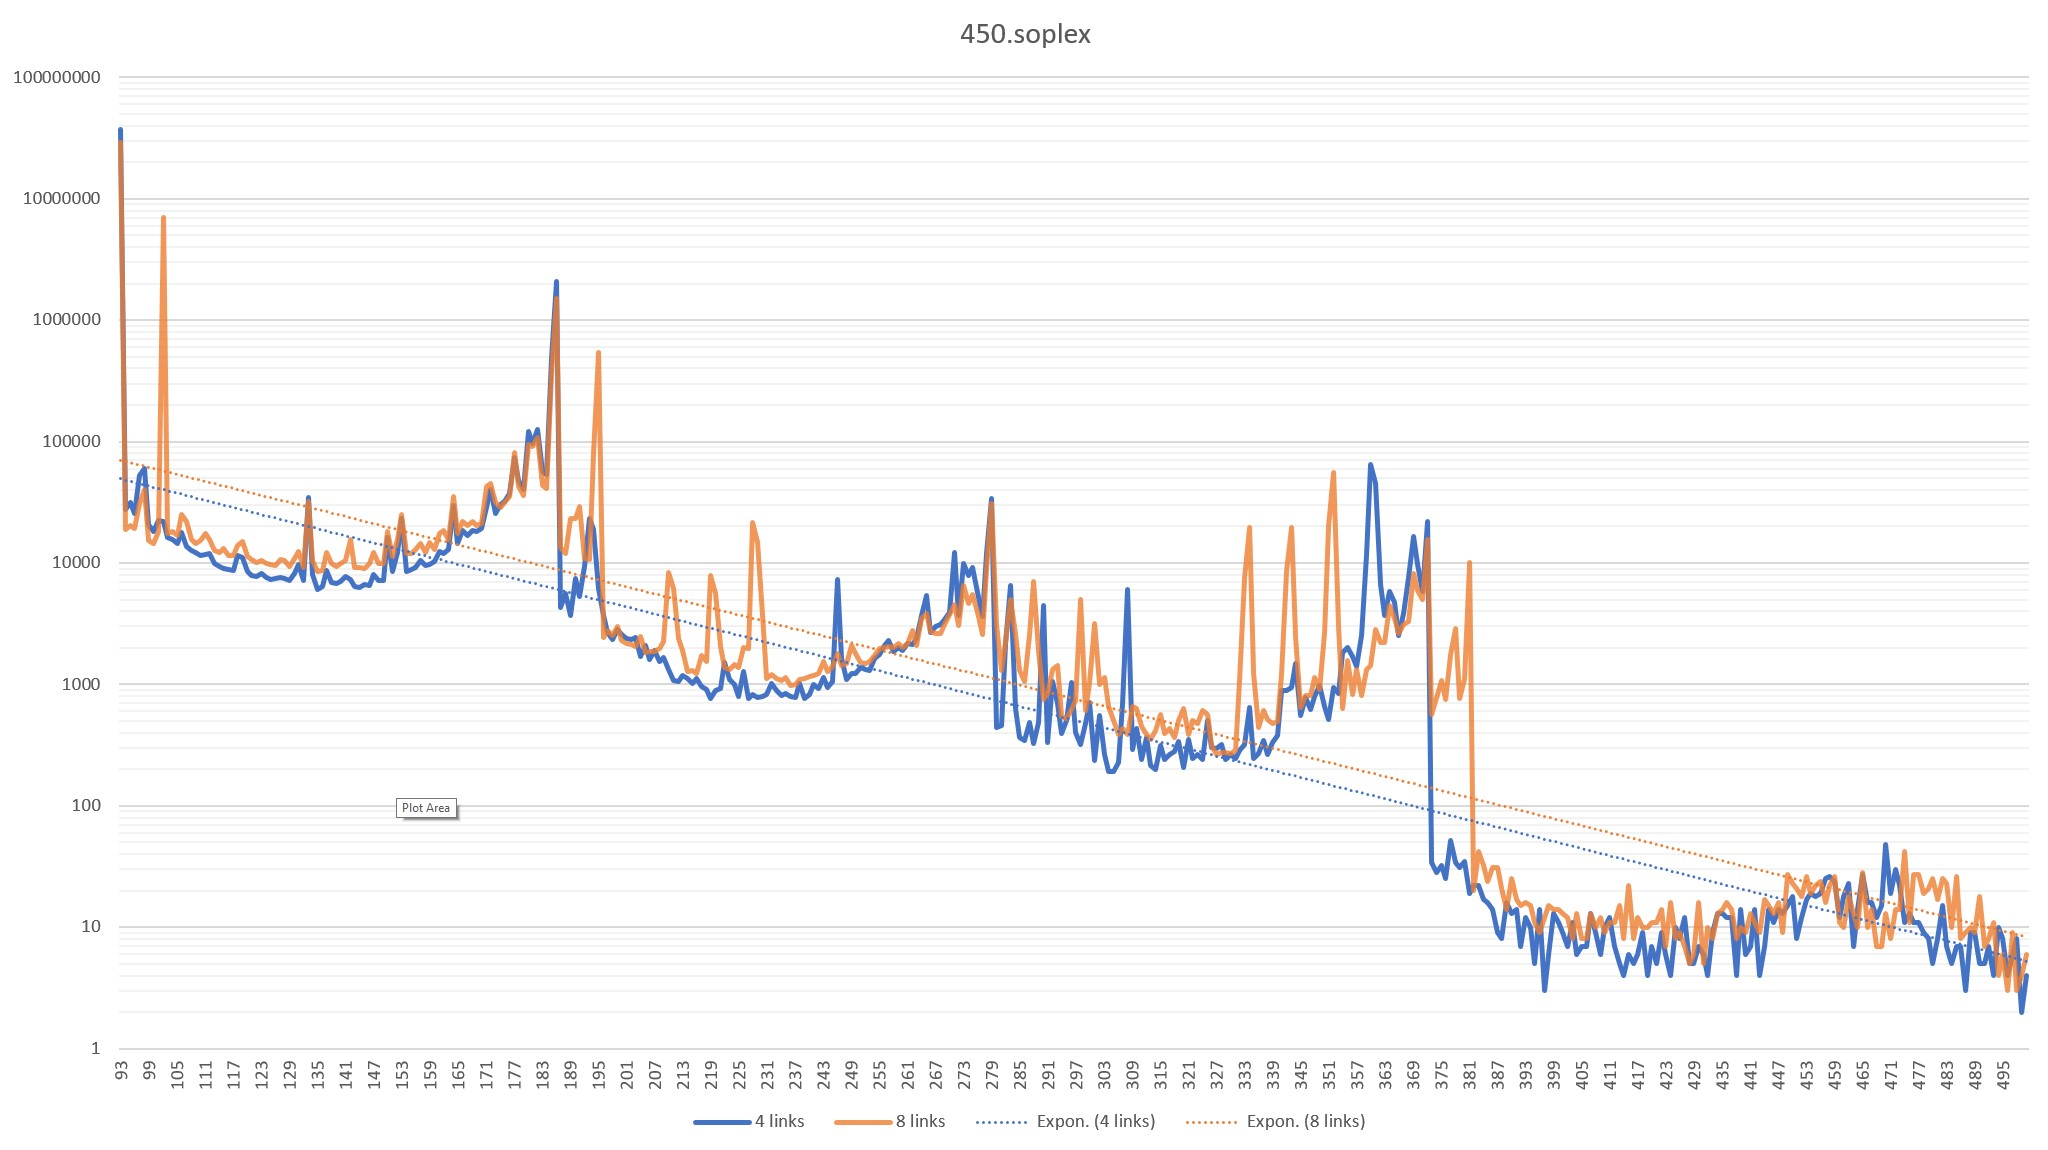
\includegraphics[width=1.0\linewidth]{figure/450-2_4-8.jpg}
    \caption{Using four links close to the processor creates additional spikes.}
    \label{Memory-access-450-2-dev-4-8-links}
\end{figure}

\section{LBM}
The results for lbm are quite similar to that of namd, except that the former has a lot more memory requests than the latter. This means that the graphs resembles one another, but the otherwise prominent peaks at 93 ns intervals start to become obscured a lot sooner with namd. Having to perform hops in the network does not affect performance significantly, as can be seen when comparing the average latencies in figure \ref{Memory-access-470-averages}. Furthermore, when studying the access pattern of different network configurations in figure \ref{Memory-access-470} we see, once again, that the patterns are very similar and that the biggest peak is at twice that of the optimal latency.
\bigskip

\begin{figure}[!ht]
    \centering
    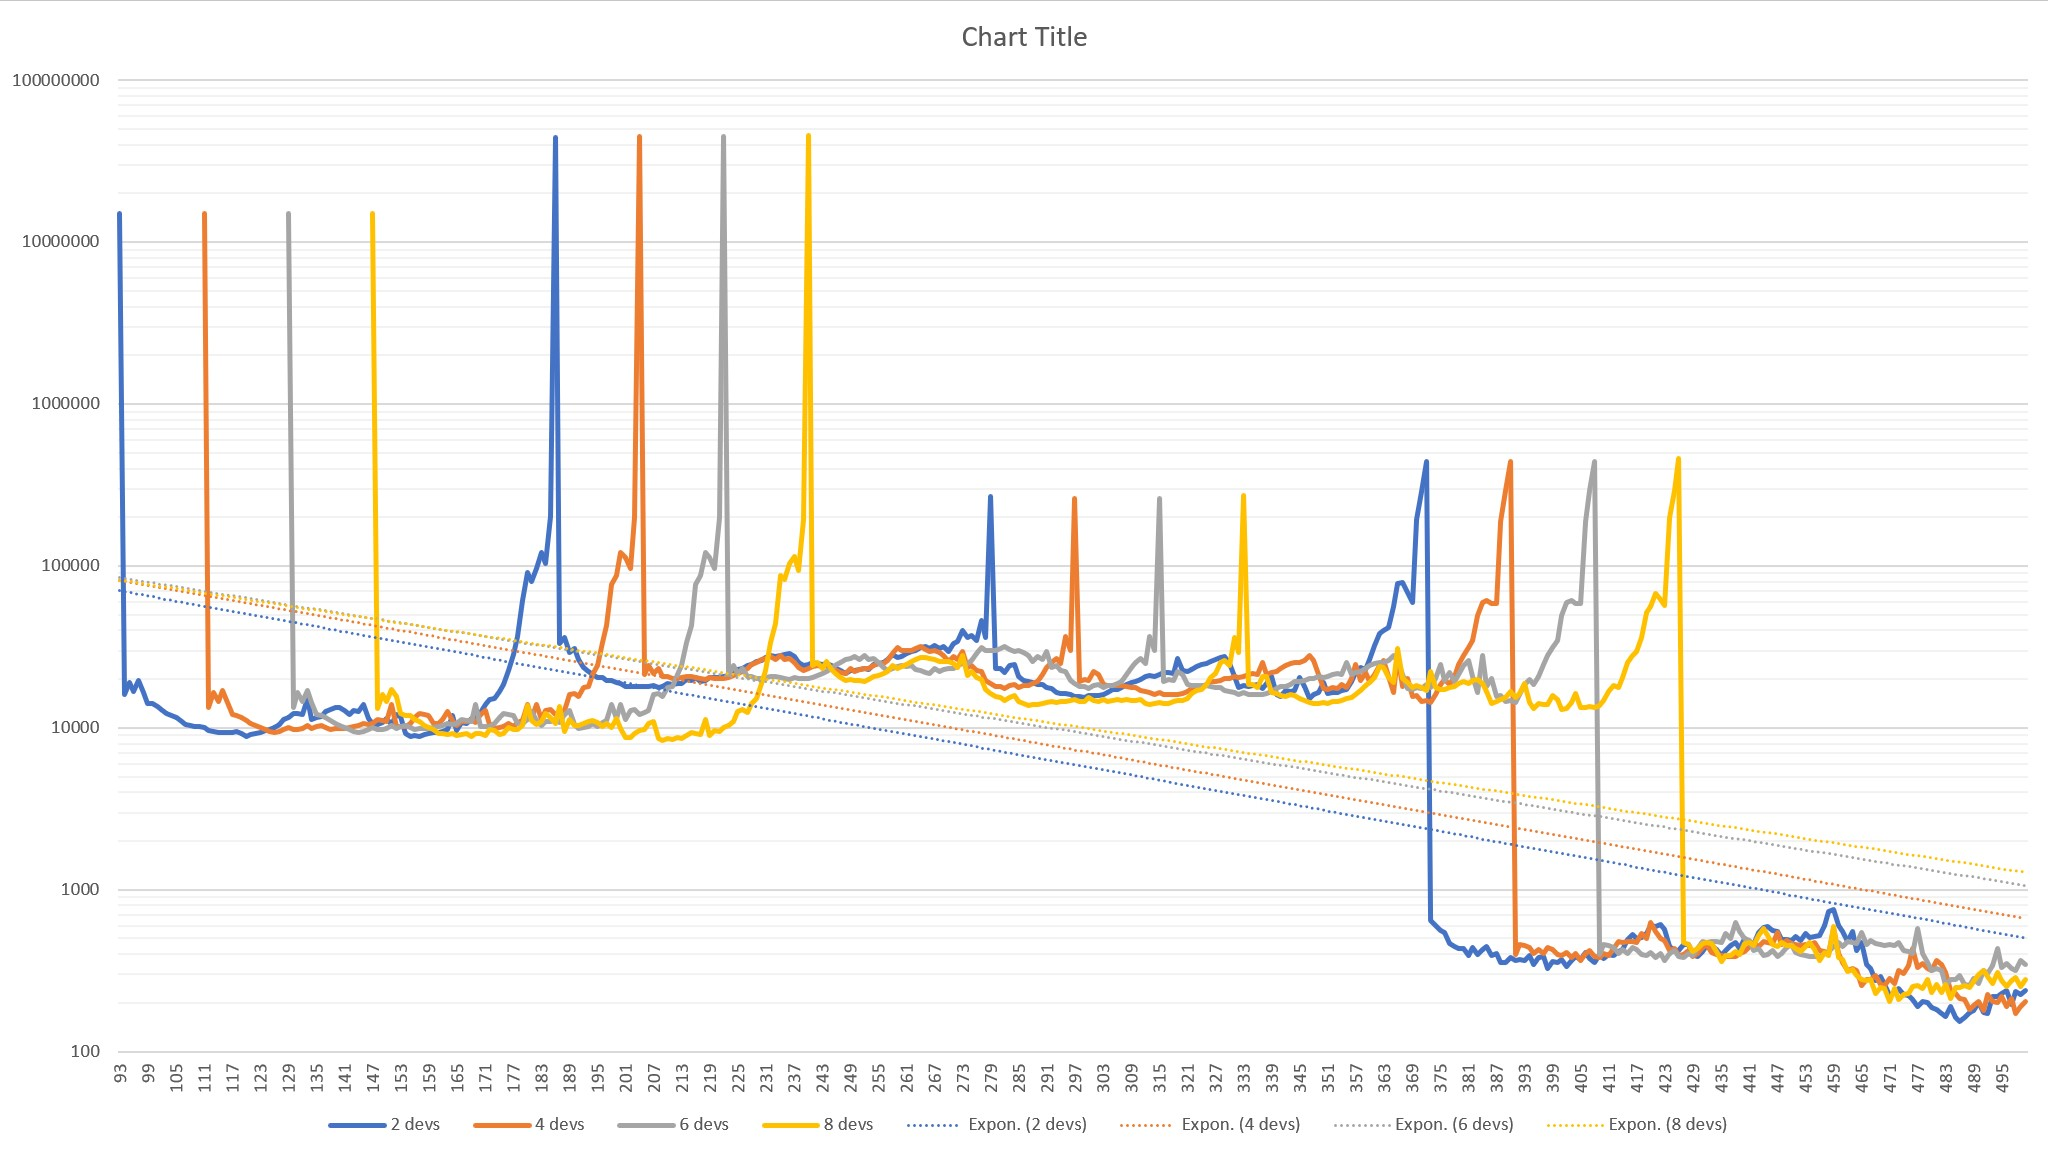
\includegraphics[width=1.0\linewidth]{figure/470-x_4.jpg}
    \caption{Access patterns between configurations.}
    \label{Memory-access-470}
\end{figure}
\begin{figure}[!ht]
    \centering
    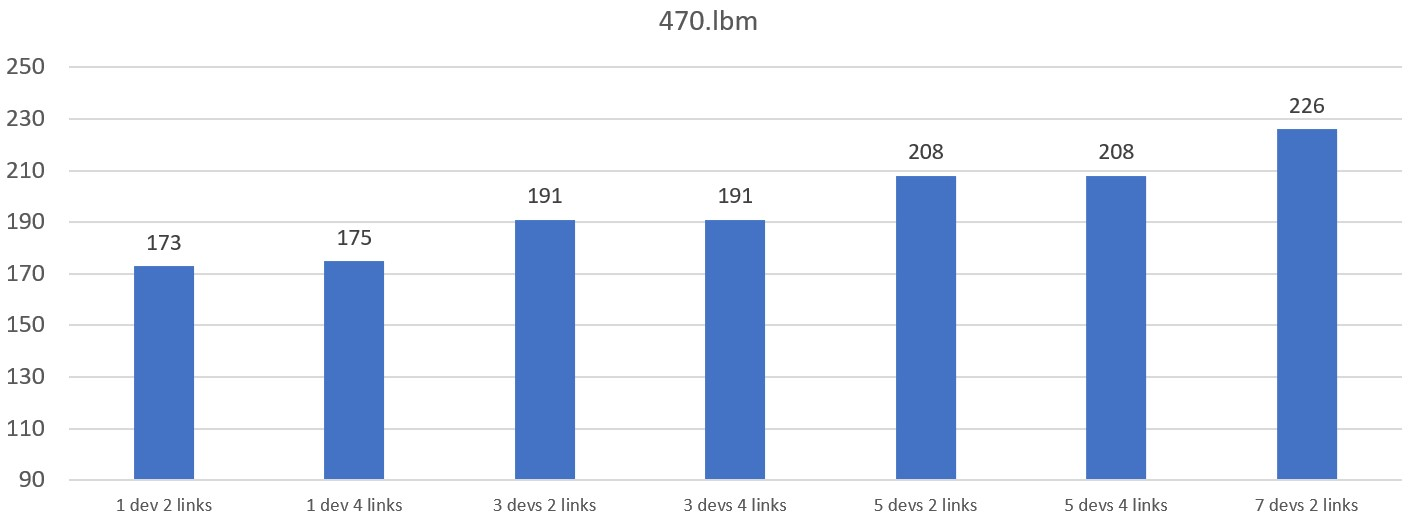
\includegraphics[width=1.0\linewidth]{figure/470-averages.jpg}
    \caption{Comparing average latencies between configurations.}
    \label{Memory-access-470-averages}
\end{figure}

The same behaviour regarding using two and four links close to the CPU, i.e. only having one device, is present when running lbm. There appears to be the same loss of performance when having to do internal routing in the first cube. Lastly, it should be noted that running lbm using four links and seven devices took too long to complete and the session was terminated without any result available. However, with the trends present among this and the other results, the outcome does not look very difficult to guess.

\section{OMNETPP}
Finally, omnetpp is run and while the results look similar to other applications there is one anomaly seen in figure \ref{Memory-access-471}. The trend lines show that there is a bigger gap between the configurations than we have seen previously, indicating that this application is causing more contention along the hops than the others have done. Since omnetpp, an application modelling large Ethernet networks, inherently supports parallelisation it might be that the application tries to do many things simultaneously. This could be conflicting with the single core host set up and could generate some waiting already at run time. 
\bigskip

\begin{figure}[!ht]
    \centering
    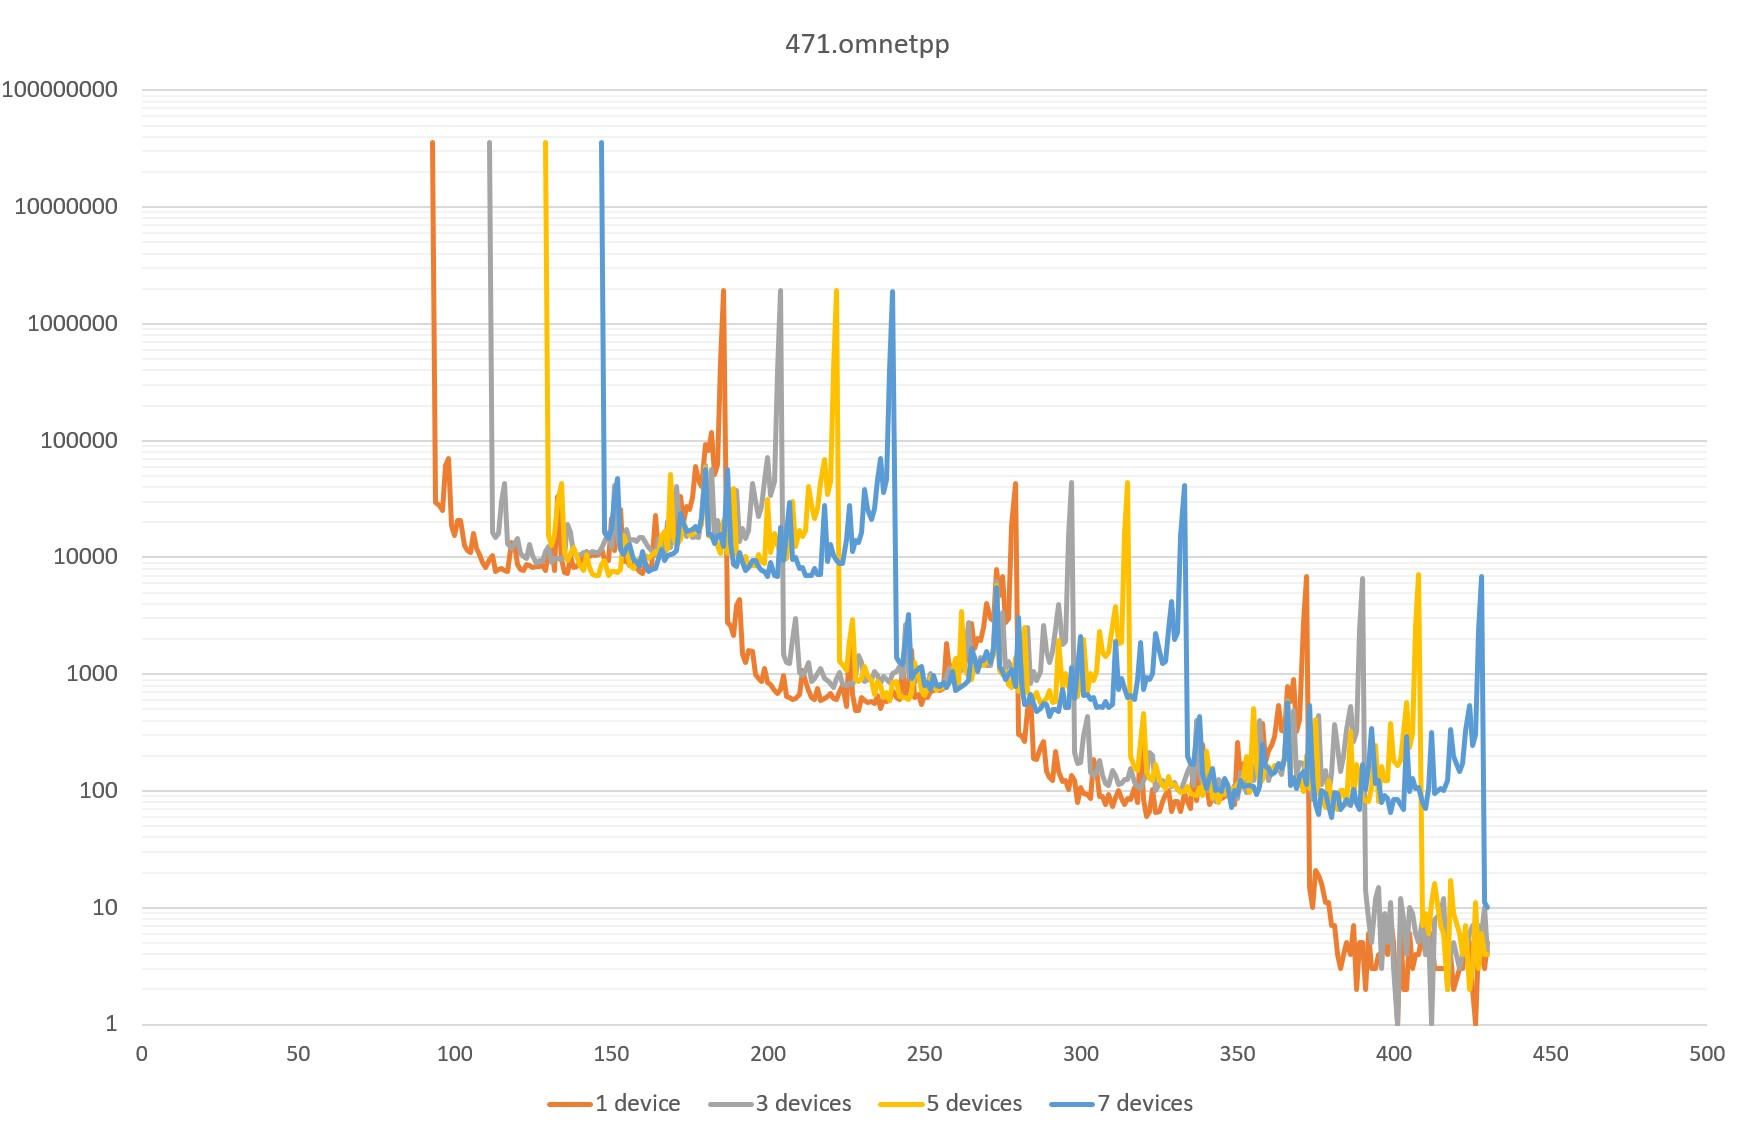
\includegraphics[width=1.0\linewidth]{figure/471-x_4.jpg}
    \caption{Access patterns between configurations.}
    \label{Memory-access-471}
\end{figure}

Viewing figure \ref{Memory-access-471-link-compare}, which compares access times using two and four links, it looks like adding MLP is unusually forgiving in terms of the size of the second spike. Comparing link configurations when having multiple hops gives more or less identical results, and the contention created by having more links available is hidden by the latency of network traversal. Despite this, the average latencies for the different setups follows a similar pattern as previous runs, as seen in figure \ref{Memory-access-471-averages}.

\begin{figure}[!ht]
    \centering
    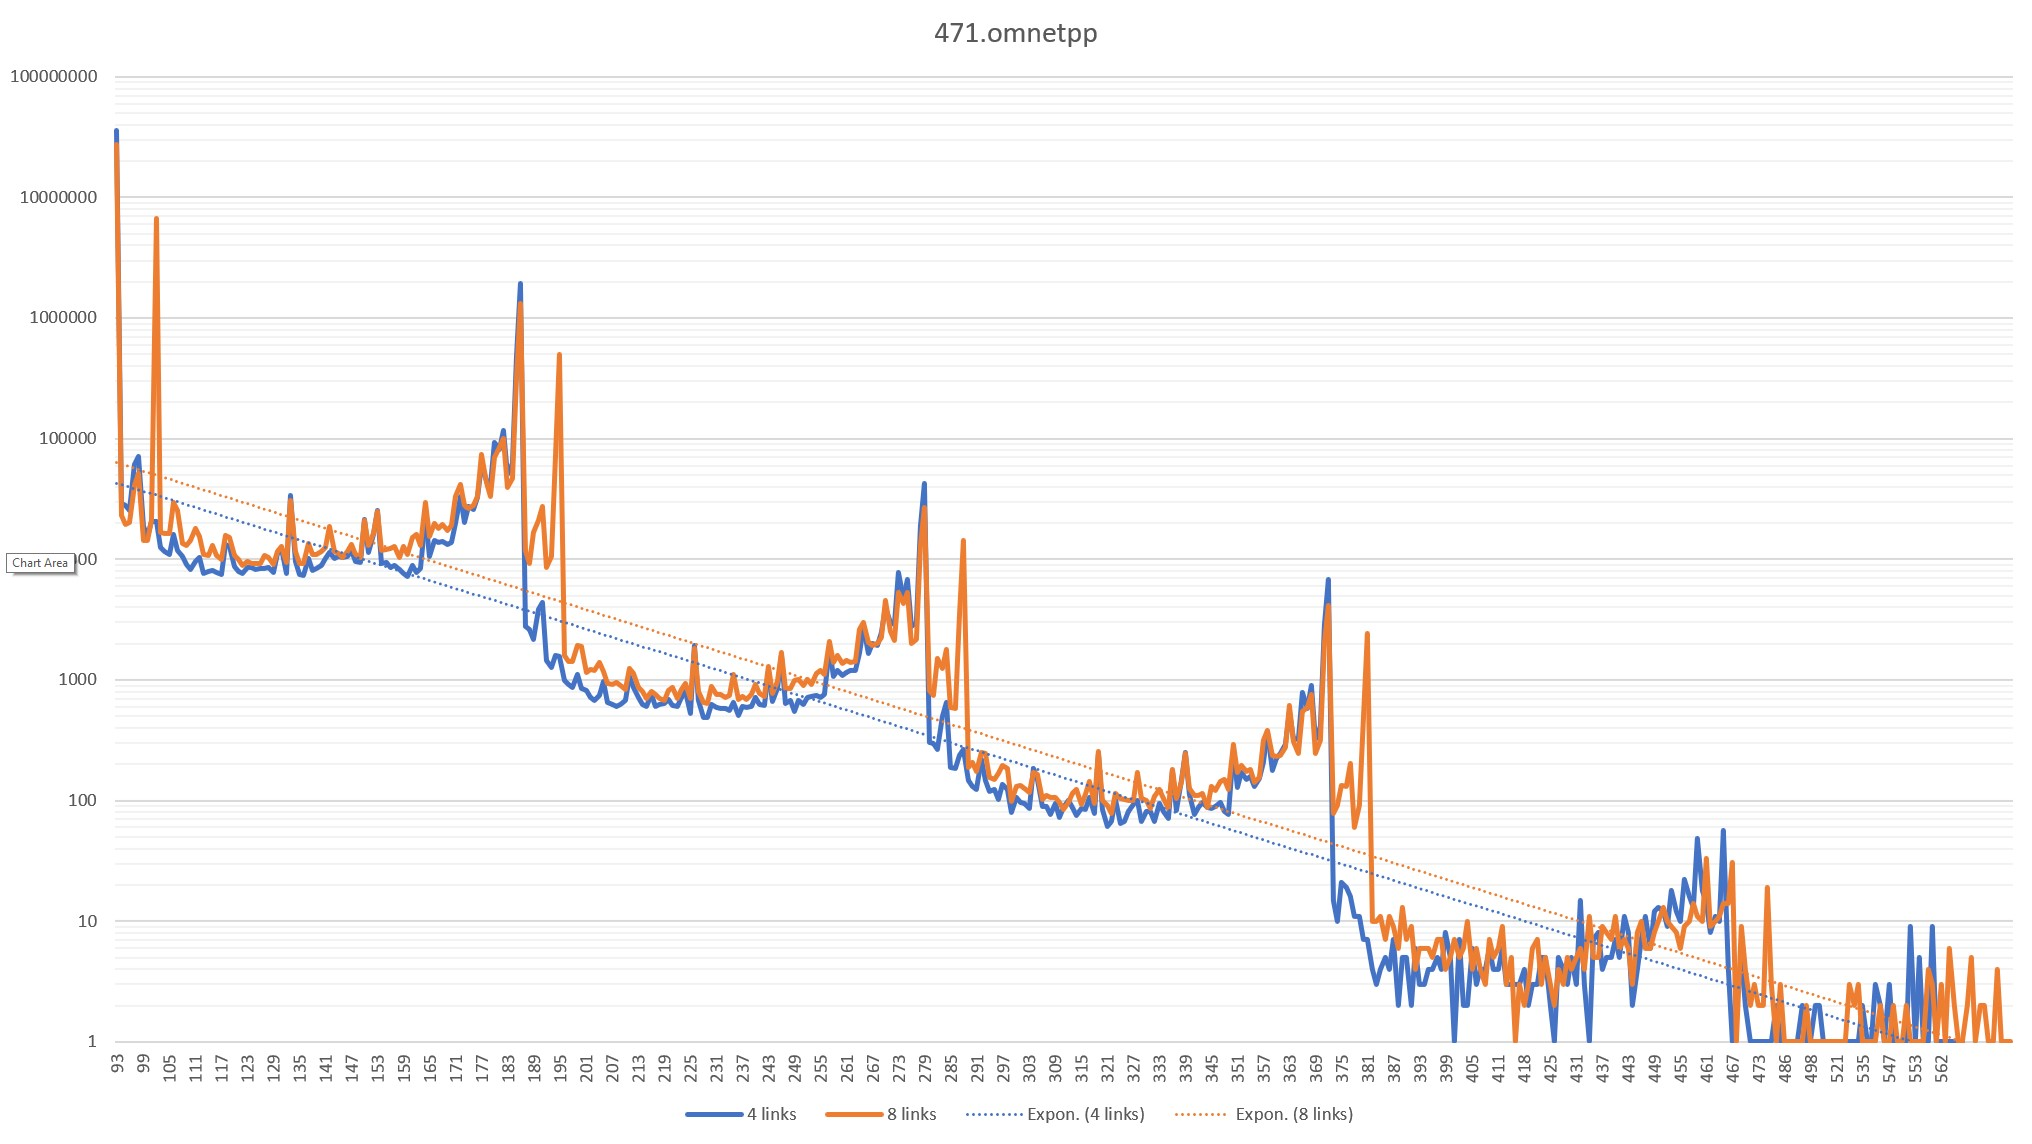
\includegraphics[width=1.0\linewidth]{figure/471-2_4-8.jpg}
    \caption{Access patterns between configurations.}
    \label{Memory-access-471-link-compare}
\end{figure}

\begin{figure}[!ht]
    \centering
    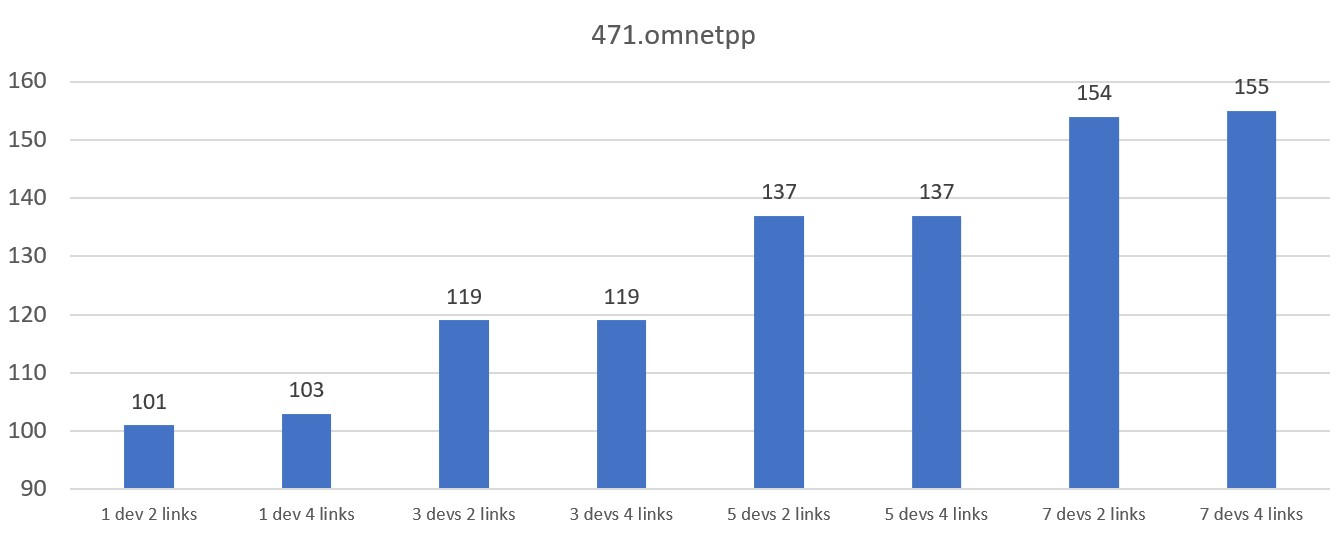
\includegraphics[width=1.0\linewidth]{figure/471-averages.jpg}
    \caption{Access patterns between configurations.}
    \label{Memory-access-471-averages}
\end{figure}

\section{Summary}
The behaviour seen between the different applications is remarkably similar. All runs provide an access latency pattern which all have the same main points. There will be an initial spike at the shortest possible latency with an arcuate, downward shape ending in another peak 93 ns later. This latter peak is either an order of magnitude bigger or smaller, depending on the application and what data and algorithm it is based on. Next there is again an arcuate shape very similar to the previous one ending in a peak 93 ns later. This repeats until there are too few memory accesses to make a comparison worthwhile. This happens regardless of how many links or cubes there are in the network, with one important exception: using two extra links, i.e. using four links, while allocating data close to processor will result in added waiting and a possible loss of performance. This could be due to the basic setup of the simulator, where the memory controller naively uses a round robin policy to check each link in turn for data, or that sending data down a link not connected to the designated vault means internal routing in the logic layer has to take place.
\bigskip

TODO: Add why the graphs look the way they do.
TODO: Unsure of context, but add that since the simulators form start mainly supported one cube, the only value avail for routing was link transfer...? 9ns. Also, with one cube requests will end up in the wrong vault, but this should have been forwarded more correctly in future cubes then

A summarised view of the average latencies can be seen in figure \ref{All-apps-latency}, where they all seem to portray the same amount of increase for each added hop. However, studying the increase in average latency in more detail, in figure \ref{All-apps-latency-trends}, we can see that some applications have a slightly higher increase than others. Specifically, mcf, which is supposed to be latency sensitive, shows that it does suffer from the longer access times. While the results obtained does seem to support this claim, it should be noted that the mcf trend line in figure \ref{All-apps-latency-trends} is based on fewer results than other applications.
\bigskip

TODO: Above section can likely be repurposed to be about correlation between latency and execution time

\begin{figure}[!ht]
    \centering
    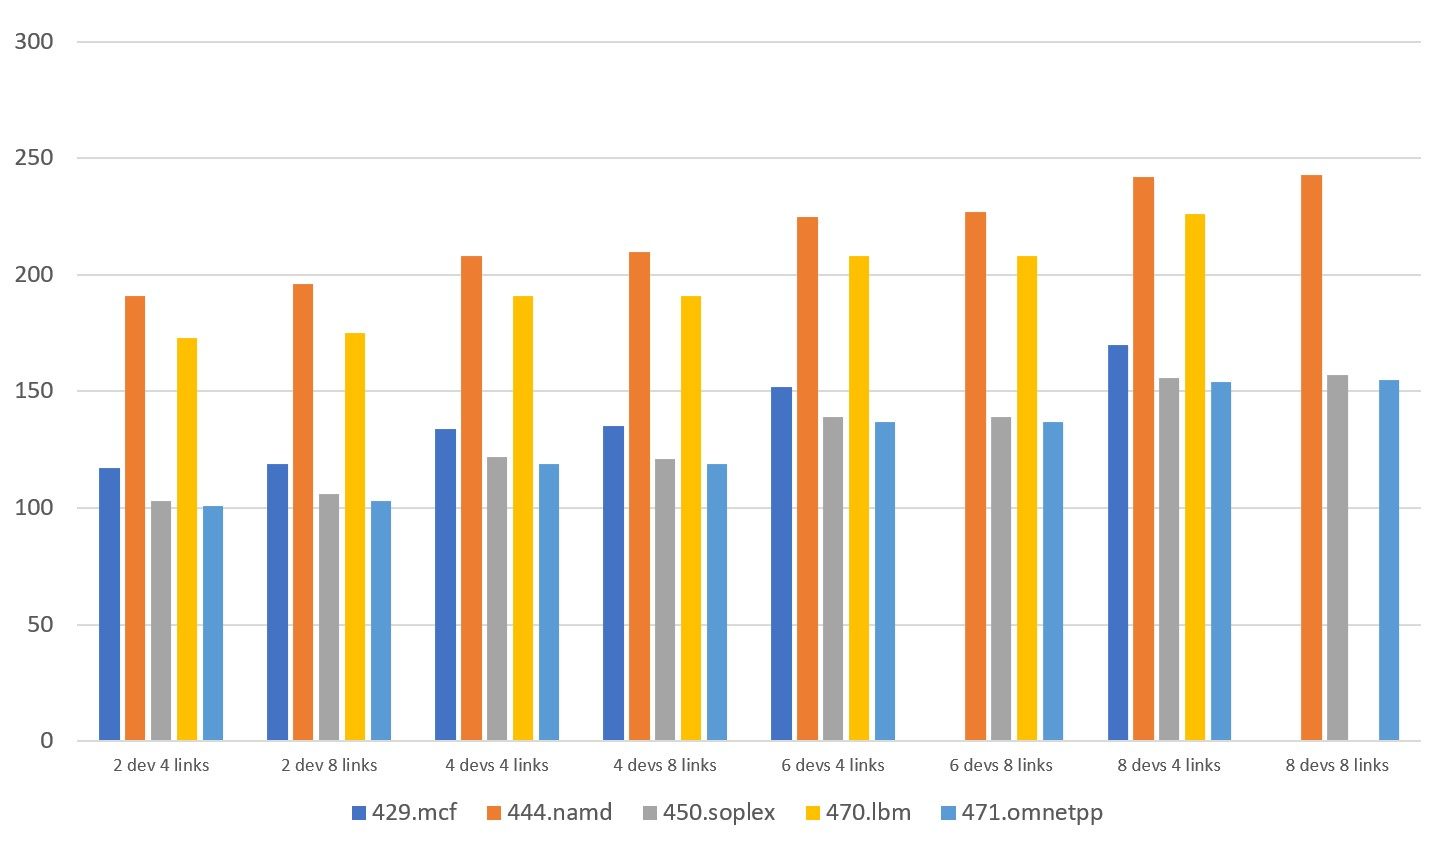
\includegraphics[width=1.0\linewidth]{figure/all-apps-latencies.jpg}
    \caption{Access patterns between configurations.}
    \label{All-apps-latency}
\end{figure}

\begin{figure}[!ht]
    \centering
    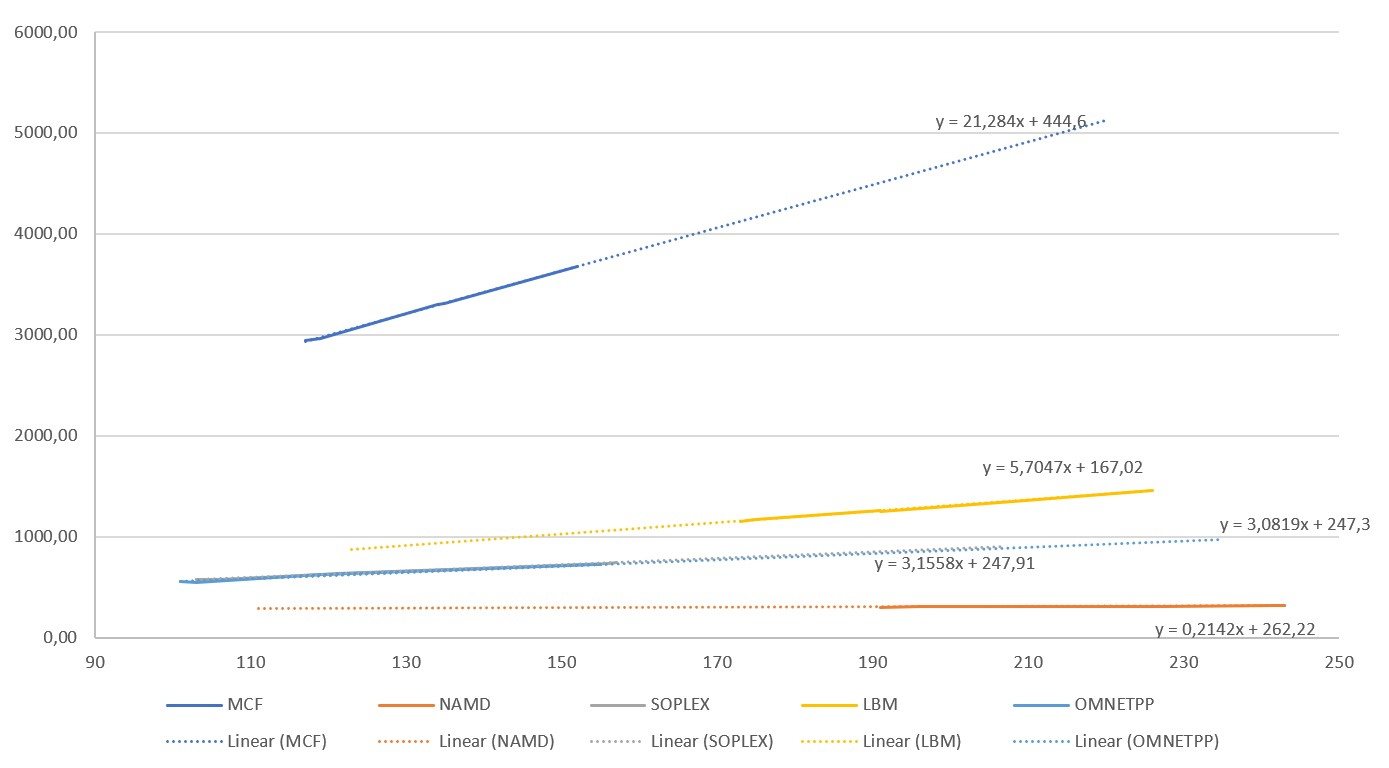
\includegraphics[width=1.0\linewidth]{figure/all-apps-latencies-trends.jpg}
    \caption{Access patterns between configurations.}
    \label{All-apps-latency-trends}
\end{figure}

Having just one HMC device in the network will let CPU get access to a high speed main memory and provides performance increases in relation to how memory bound an application is, similar to that of having a normal DDRx memory available albeit at a lower bandwidth. One of the biggest differences lies in the fact that the memory controller when using HMC is placed beneath the memory stack. There is an advantage in bus utilisation where having HMC's abstract network layer decreases the number of trips to host. Traditionally, CPUs need to determine if something is a pointer, consult the TLB if it is present and otherwise access main memory for it. With this approach, we instead leave out the extra trip back to CPU and instead allow the memory controller (logic layer) to determine this. This helps reduce contention created by pointer chasing.
\bigskip

Finally, all of these results were attained on a very simple host system in order to minimise complexity. The virtual cores used by Ariel appear, in hindsight, to be in-order, which might make MLP hard to exploit. When an instruction pipeline has to stall entirely while waiting for data from the memory, it is difficult to schedule data in a way where multiple memory requests can be in-flight simultaneously. This could also explain why the benchmarks all behave quite similar when it comes to access times.
